
\chapter{FOUNDATION Fieldbus instrumentation}

\label{Foundation_Fieldbus}

\textit{FOUNDATION Fieldbus} is a standard for digital field instrumentation enabling field instruments to not only communicate with each other digitally, but also to execute all continuous control algorithms (such as PID, ratio control, cascade control, feedforward control, etc.) traditionally implemented in dedicated control devices.  In essence, FOUNDATION Fieldbus extends the general concept of a distributed control system (DCS) all the way to the field devices themselves.  In this way, FOUNDATION Fieldbus sets itself apart as more than just another digital communication ``bus'' for industry -- it truly represents a new way to implement measurement and control systems.  This chapter is devoted to a discussion of FOUNDATION Fieldbus instrumentation, building on general concepts of digital data acquisition and communication previously explored in this book.  \index{FOUNDATION Fieldbus}

For brevity, ``FOUNDATION Fieldbus'' will be abbreviated as \textit{FF} throughout the rest of this chapter.  \index{FF (FOUNDATION Fieldbus)}

\vskip 10pt

This particular industrial network standard was first proposed as a concept in 1984, and officially standardized by the Fieldbus Foundation (the organization overseeing all FF standards and validation) in 1996.  To date, adoption of FF has been somewhat slow, mostly limited to new construction projects.  One of the ``selling points'' of FF is decreased installation time, which makes it a more attractive technology for brand-new installations than for retrofit projects.







\filbreak
\section{FF design philosophy}

To understand just how different FOUNDATION Fieldbus is from other digital instrument systems, consider a typical layout for a distributed control system (DCS), where all the calculations and logical ``decisions'' are made in dedicated \textit{controllers}, usually taking the form of a multi-card ``rack'' with processor(s), analog input cards, analog output cards, and other types of I/O (input/output) cards:

$$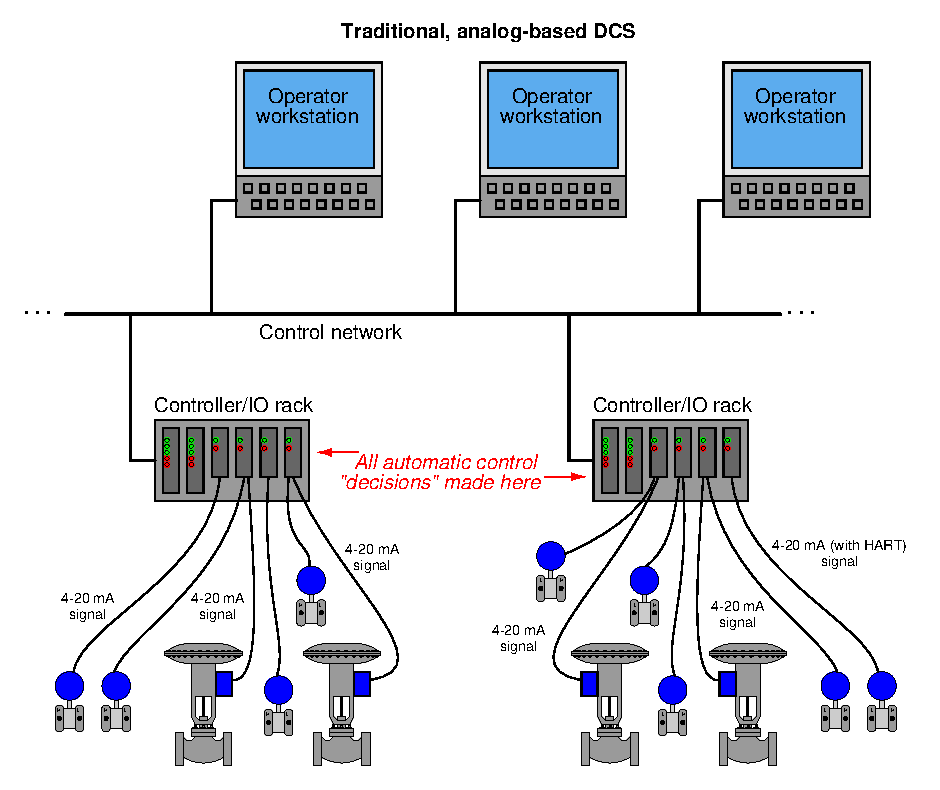
\includegraphics{fieldbus_01.eps}$$

Information is communicated in analog form between the DCS controllers and the field instruments.  If equipped with the proper types of I/O cards, the DCS may even communicate digitally with some of the field instruments using \textit{HART} protocol.  This allows remote configuration and diagnostic testing of field instruments from the host system, or from anywhere along the cable when using a hand-held HART communicator.

\filbreak

It is even possible to build a control system around a DCS using all digital field instruments, using a protocol such as \textit{Profibus PA} to exchange process variable (PV) and manipulated variable (MV) signals to and from the DCS controllers at digital speeds far exceeding that of HART:  \index{Profibus PA}

$$\includegraphics{fieldbus_02.eps}$$

Now, multivariable field instruments have the ability to quickly exchange their data with the DCS, along with maintenance-related information (calibration ranges, error messages, and alarms).  Each ``fieldbus'' cable is a multi-drop digital network, permitting multiple field devices per cable and consequently reducing total cable length and connection count.  \textit{Coupling devices} may be used in lieu of terminal blocks to conveniently connect multiple instruments together on common networks leading to the DCS.  Still, however, all the automatic control algorithms are implemented in the DCS.

\filbreak

A FOUNDATION Fieldbus system goes one step further by allowing all control algorithms to be executed within the field instruments rather than relying on the DCS controllers to make automatic control ``decisions.''  In fact, the DCS would not even be necessary if not for the need of operations personnel to monitor and alter control system status:

$$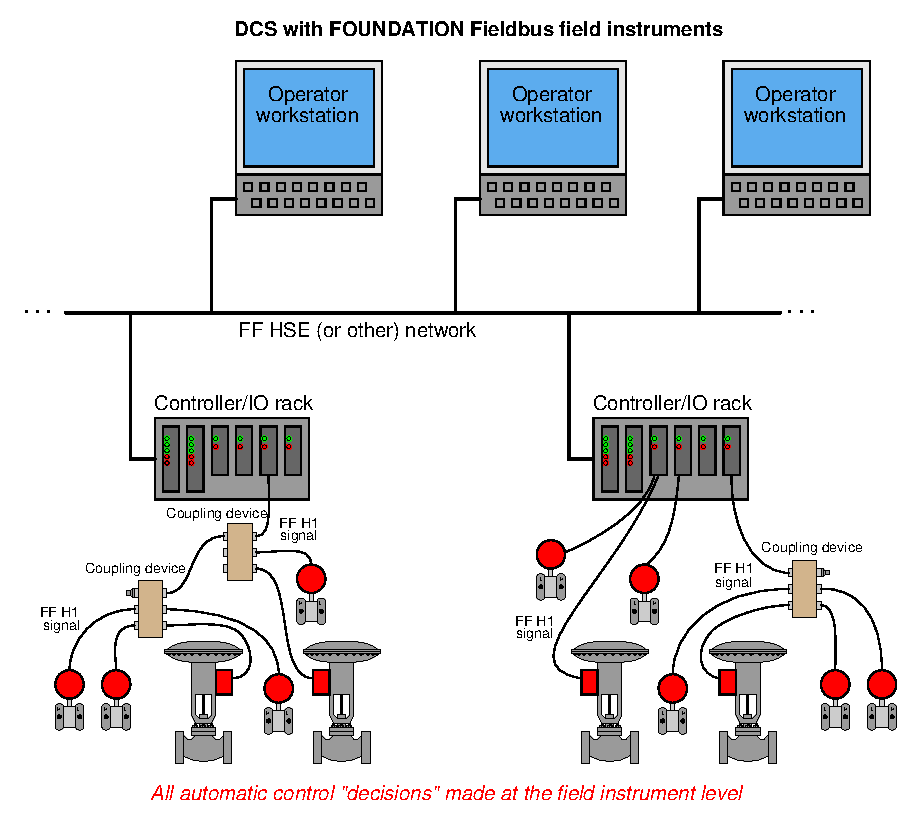
\includegraphics{fieldbus_03.eps}$$

That being said, it is possible (and in fact common) for control algorithms to be placed in the DCS controllers in addition to algorithms executed by FF field devices.

\filbreak

The locations of the control algorithms -- those microprocessor instructions dictating how the loop will be controlled -- in these different systems deserves further elaboration.  To show this, I will make use of \textit{function block} notation to show where the algorithms are executed in each system type, each function block shown as a yellow box on the diagram.  

First, the DCS with analog I/O (inputs/outputs):

$$\includegraphics{fieldbus_41.eps}$$

The conversion of 4-20 mA signals from transmitters into a scaled digital number values inside the DCS takes place inside ``analog input'' (AI) function blocks programmed into the DCS.  These converted values then pass to PID function blocks where the arithmetic for control loop decisions takes place.  Finally, the digital output values of the PID blocks get passed on to ``analog output'' (AO) function blocks where those values are converted back into 4-20 mA analog signals to drive control valves, variable-frequency drives (VFDs), and other final control elements.  Each ``function block'' is nothing more than a segment of programming code instructing the DCS's microprocessor what to do with the signal values.  Function blocks are usually selected and arranged by engineers and technicians maintaining the DCS using graphical programming software, allowing function blocks to be placed onto a ``palette'' and connected with lines to show where their signals come from and go to.  \index{Variable-frequency drive}  \index{VFD}

\filbreak

Now let us examine Profibus PA again.  Here, the field instruments are entirely digital, communicating with each other via digital signals over a network cable to the DCS.  This means none of the cables carry analog signals anymore, necessitating the A/D and D/A conversion take place inside the field devices themselves.  It also means we may do away with the old analog I/O cards in the DCS rack, replacing them with a single network interface card:

$$\includegraphics{fieldbus_42.eps}$$

Control decisions still take place within the DCS microprocessor, which is why the PID function blocks are still shown inside the processor card.  The analog-digital signal conversions and scaling operations, however, occur within the field instruments themselves.  Such is the nature of digital networks that multiple instruments may share the same communication cable back to the DCS, with each instrument ``taking turns'' communicating in time.

\filbreak

FOUNDATION Fieldbus, by contrast, allows even the control decisions to take place within the field devices, unburdening the DCS to perform higher-level tasks as necessary:

$$\includegraphics{fieldbus_43.eps}$$

With each evolutionary step in system design, the trend has been to ``push'' the control algorithms further into the field, away from the central control system.  FOUNDATION Fieldbus is the ultimate realization of this trend, where the field instruments themselves can do all necessary control functions.  Here, the only necessary purposes served by the DCS are:

\begin{itemize}
\item Initial configuration and maintenance tool for the FF instruments
\item Provide operators with an interface allowing indication and adjustment of control parameters
\item Record long-term ``historical'' data on the process being controlled
\end{itemize}

In fact, given the right FF system design, the DCS could even be \textit{disconnected} from the FF network, and the FF instruments would continue to control the process as they did before!

\filbreak

This is not to say that all control algorithms \textit{must} be executed within the field instruments in a FOUNDATION Fieldbus control system.  In fact it is quite common to find FF control systems implemented with the host (DCS) performing most of the control.  FOUNDATION Fieldbus permits but does not mandate that all control tasks reside ``in the field''.

\vskip 10pt

When the FF standard was being designed, two different network levels were planned: a ``low speed'' network for the connection of field instruments to each other to form network \textit{segments}, and a ``high speed'' network for use as a plant-wide ``backbone'' for conveying large amounts of process data over longer distances.  The low-speed (field) network was designated \textit{H1}, while the high-speed (plant) network was designated \textit{H2}.  Later in the FF standard development process, it was realized that existing Ethernet technology would address all the basic requirements of a high-speed ``backbone,'' and so it was decided to abandon work on the H2 standard, settling on an extension of 100 Mbps Ethernet called \textit{HSE} (``High Speed Ethernet'') as the backbone FF network instead.  \index{FOUNDATION Fieldbus H1}  \index{FOUNDATION Fieldbus H2}   \index{FOUNDATION Fieldbus HSE}  \index{Ethernet}

\vskip 10pt

The bulk of this chapter will focus on H1 rather than HSE.









\filbreak
\section{H1 FF Physical layer}

Layer 1 of the OSI Reference Model is where we define the ``physical'' elements of a digital data network.  The H1 FF network exhibits the following properties:

\begin{itemize}
\item Two-wire (ungrounded) network cable
\item 100 ohm (typical) characteristic impedance
\item DC power is conveyed over the same two wires as digital data
\item 31.25 kbps data rate
\item Differential voltage signaling (0.75 volts peak-to-peak transmit minimum ; 0.15 volts peak-to-peak receive threshold minimum)
\item Manchester encoding
\end{itemize}

Since DC power is conveyed over the same two wires as the digital data, it means each device only needs to connect to two wires in order to function on an H1 network segment.  The choice of a (relatively) slow 31.25 kbps data rate allows for imperfect cables and terminations which would otherwise plague a faster network.  Manchester encoding embeds the network clock pulse along with the digital data, simplifying synchronization between devices.

As you can see, the layer 1 design parameters were chosen to make FF H1 networks easy to build in unforgiving industrial environments.  The physical layer of FOUNDATION Fieldbus happens to be identical to that of Profibus-PA, further simplifying installation by allowing the use of common network validation tools and connection hardware.





\filbreak
\subsection{Segment topology}

A minimal FF H1 segment consists of a DC power supply, a ``power conditioner,'' exactly two terminator resistors\footnote{Each FF terminator resistor is actually a series resistor/capacitor network.  The capacitor blocks direct current, so that the 100 $\Omega$ resistor does not impose a DC load on the system.  The substantial current that would be drawn by a 100 ohm resistor across 24 VDC source if not blocked by a series capacitor (24 V / 100 ohms = 240 mA) would not only waste power (nearly 6 watts per resistor!) but that much current would cause an unnecessary degradation of supply voltage at the field device terminals due to voltage drop along the length of the segment cable's conductors.} (one at each extreme end of the cable), a shielded and twisted-pair cable, and of course at least two FF instruments to communicate with each other.  The cable connecting each instrument to the nearest junction is called a \textit{spur} (or sometimes a \textit{stub} or a \textit{drop}), while the cable connecting all junctions to the main power source (where a host DCS would typically be located) is called a \textit{trunk} (or sometimes a \textit{home run} for the section leading directly to a host system):  \index{Stub}  \index{Spur}  \index{Drop}

$$\includegraphics{fieldbus_04.eps}$$

The power conditioner shown in this diagram is a simplified model of the actual device, the function of which being to filter out digital data pulses from reaching the DC power supply.  Commercially-available Fieldbus power conditioners are complex electronic circuits rather than passive filter networks.

Normally, we would find more than two FF devices connected to a trunk cable, as well as a ``host'' system such as a DCS FF card for accessing FF instrument data, performing maintenance tasks, and integrating with other control loops.  Regardless of how many (or how few) FF devices connect to an H1 segment, though, there should always be \textit{exactly two} terminating resistors in each segment -- one at each end\footnote{Be sure to check the specifications of the host system H1 interface card, because many are equipped with internal terminating resistors given the expectation that the host system will connect to one far end of the trunk!} of the trunk cable.  These resistor/capacitor networks serve the sole purpose of eliminating signal reflections off the ends of the trunk cable, making the cable look infinitely long from the perspective of the propagating pulse signals.  Missing terminators will result in signal reflections off the unterminated line end(s), while extra terminators have the equally deleterious effect of attenuating signal strength (as well as potentially causing signal reflections of opposite phase).

\filbreak

All H1 networks are essentially parallel electrical circuits, where the two connection terminals of each field instrument are paralleled to each other.  The physical arrangement of these transmitters, though, may vary substantially.  The simplest way to connect FF H1 devices together is the so-called ``daisy-chain'' method, where each instrument connects to two cable lengths, forming an uninterrupted ``chain'' network from one end of the segment to the other:

$$\includegraphics{fieldbus_05.eps}$$

As simple as this topology is, it suffers from a major disadvantage: it is impossible to disconnect any device in the segment without interrupting the network's continuity.  Disconnecting (and reconnecting for that matter) any device necessarily results in all ``downstream'' devices losing signal, if only for a brief time.  This is an unacceptable liability in most industrial applications, as it complicates maintenance and servicing of individual instruments on the segment.

\filbreak

An alternative topology is the \textit{bus} layout, where short ``spur'' cables connect instruments to a longer ``trunk'' cable.  Terminal blocks -- or even quick-disconnect couplings -- within each junction box provide a convenient means of disconnecting individual devices from the segment without interrupting data communication with the other devices:

$$\includegraphics{fieldbus_06.eps}$$

The ideal arrangement for a ``bus'' network is to minimize the length of each spur cable, so as to minimize the delay of reflected signals off the unterminated ends of the drops.  Remember that only \textit{two} termination resistors are allowed in any electrically continuous network segment, and so this rule forbids the addition of terminators to the end of each spur cable.  

\filbreak

Yet another alternative topology for H1 networks is the so-called \textit{chicken-foot} arrangement, where a long trunk cable terminates at a multi-point junction along with several field devices and their spur cables:

$$\includegraphics{fieldbus_07.eps}$$

Most FF systems resemble a combination of ``bus'' and ``chicken-foot'' topologies, where multiple junction devices serve as connection points for two or more field instruments per junction.  




\filbreak
\subsection{Coupling devices}

In order to simplify the task of connecting Fieldbus devices to such a network segment, multiple manufacturers sell \textit{coupling devices} (often informally referred to as \textit{bricks}) with quick-disconnect electrical fittings so the end-user does not have to build and commission junction boxes using standard terminal blocks.  A photograph of a Turck brand Fieldbus coupling device appears here, showing multiple spur cables plugged into it:  \index{Turck Fieldbus coupling device}  \index{Coupling device, fieldbus}  \index{Brick, Fieldbus coupler}

$$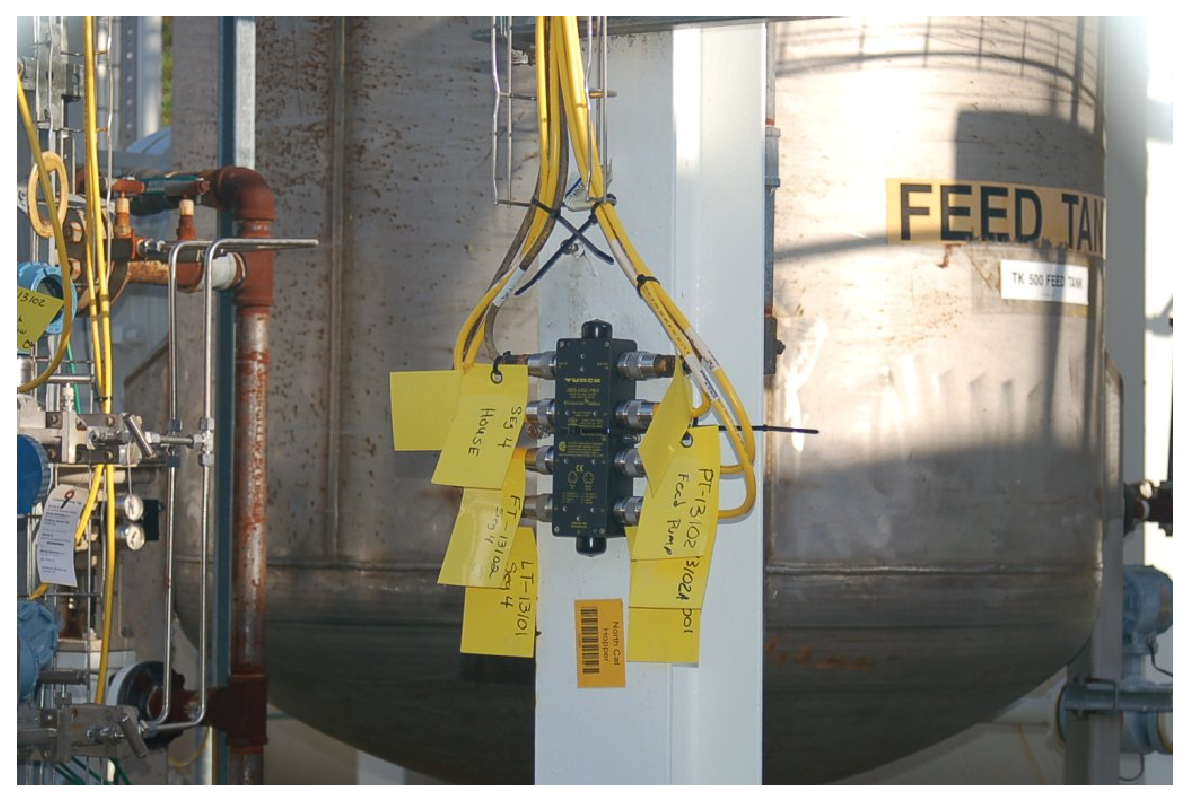
\includegraphics[width=4in]{fieldbus_08.eps}$$

Coupling devices are highly recommended for all industrial fieldbus systems, FF or otherwise.  Not only do these devices provide a convenient means of forming highly reliable connections between field instruments and the trunk cable, but many of them are equipped with features such as short-circuit protection (so that a shorted spur cable or field instrument does not cause the entire segment to stop communicating) and LED indication of spur status.

Cables connecting to a coupling device must be equipped with special plugs matching the sockets on the coupler.  This presents a bit of a problem when attempting to pull such a cable through electrical conduit: the bulky plug requires either over-sized conduit to accommodate the plug's width, or requires the plug be installed on the cable after pulling through the conduit.  Both approaches are expensive, the first in terms of capital cost and the second in terms of installation labor.  For this reason, many installers abandon electrical conduit altogether in favor of \textit{ITC} (``Instrument Tray Cable'').

\filbreak

A wider-angle photograph of the coupling device previously shown reveals many ITC cables and their routing through wire ``basket'' style trays among process instruments and vessels:  \index{ITC}  \index{Instrument tray cable (ITC)}

$$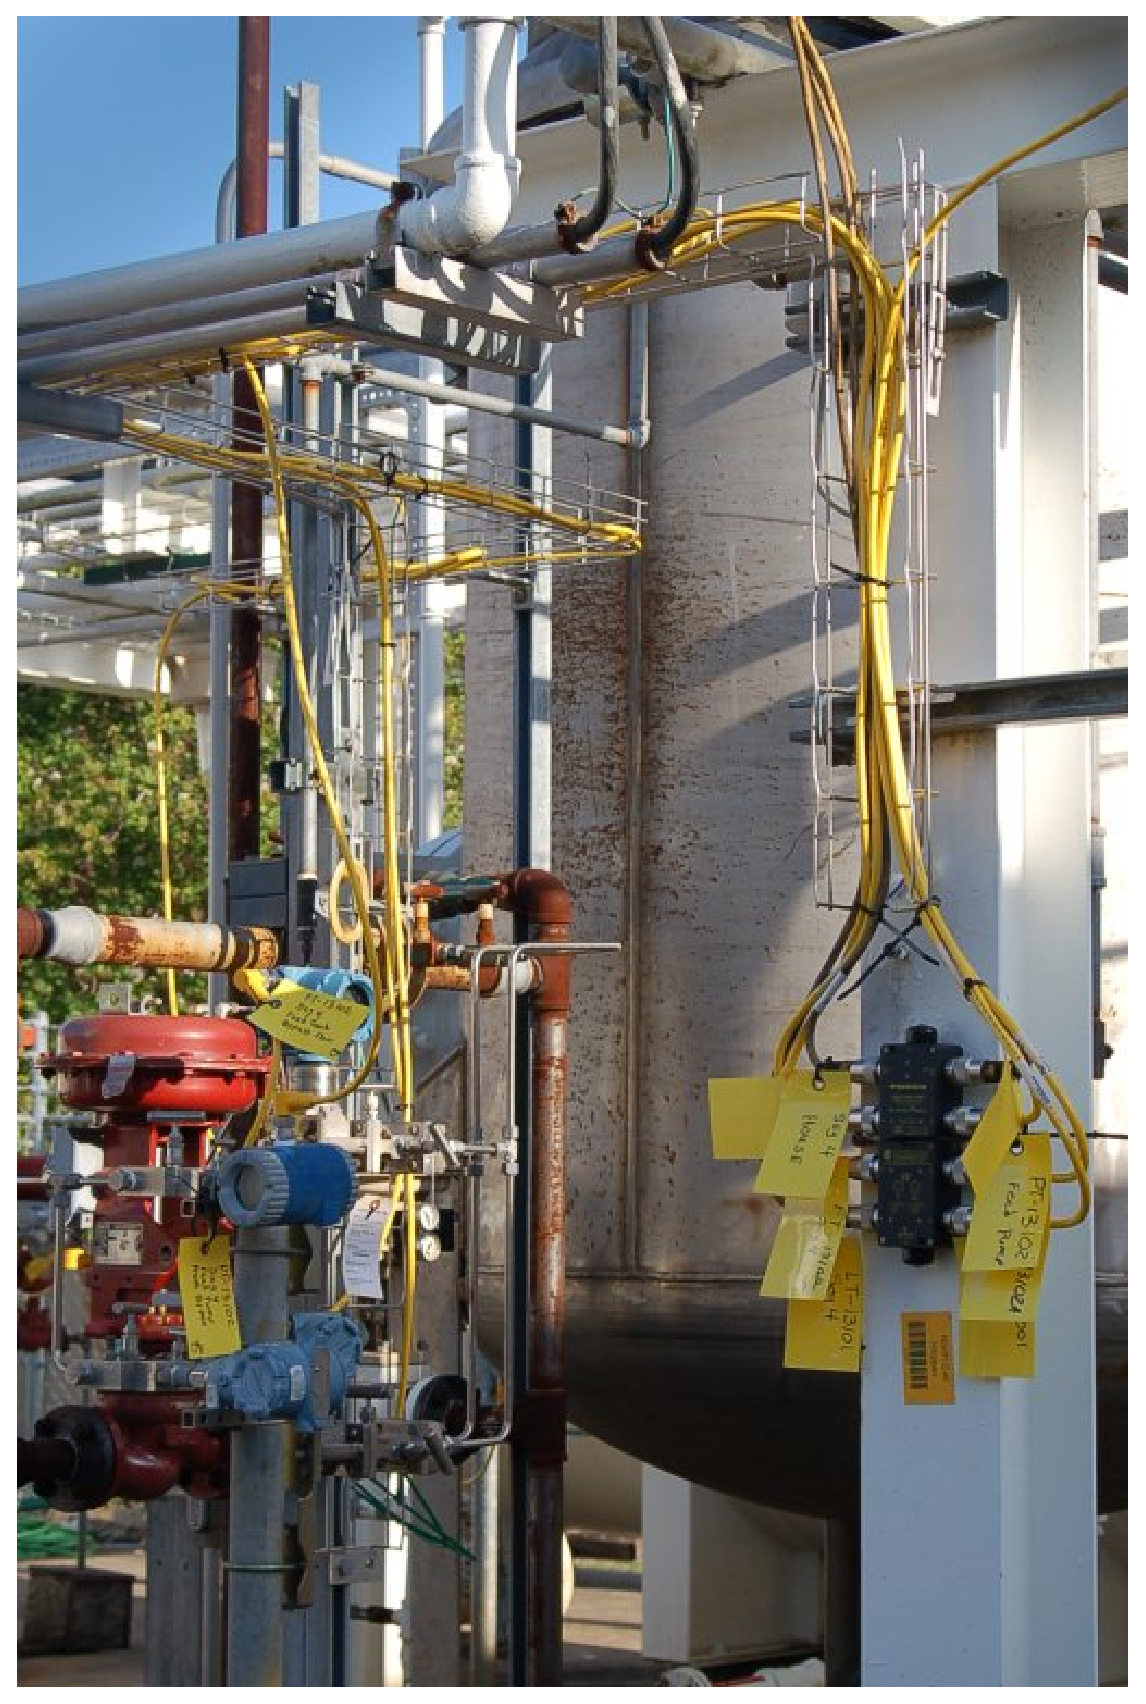
\includegraphics[width=3in]{fieldbus_09.eps}$$

As evident in this photograph, ITC is obviously rated for continuous exposure to direct sunlight and moisture, as well as a certain amount of physical distress (abrasion, high and low temperatures, etc.).  Article 727 of the National Electrical Code (NEC) defines the acceptable uses and installations of ITC\footnote{You should consult an NEC code book regarding specific limitations of ITC wiring.  Some of the main points include limiting individual ITC cable lengths to a maximum of 50 feet, and mechanically securing the cable at intervals not to exceed 6 feet.}.  \index{National Electrical Code (NEC)}  \index{NEC}

It should be noted that while a properly shielded and grounded FF cable is quite resistant to radio-frequency interference, coupling devices may present ``weak spots'' where radio interference may find its way onto the segment.  Different styles of coupling devices offer differing levels of immunity to RF (Radio Frequency) noise.  Those made of metal and properly bonded to ground will be well-shielded, while those made of plastic having exposed connection terminals offer little or no protection.  In any case, it is a good practice to avoid ``keying'' any portable radio transmitter in the near vicinity of a Fieldbus coupling device.  \index{Radio Frequency (RF)}  \index{RF}

\filbreak

Not all Fieldbus couplers are rated for outdoor installation.  Some are intended for mounting inside electrical enclosures, such as this Pepperl+Fuchs model shown mounted on a DIN rail:

$$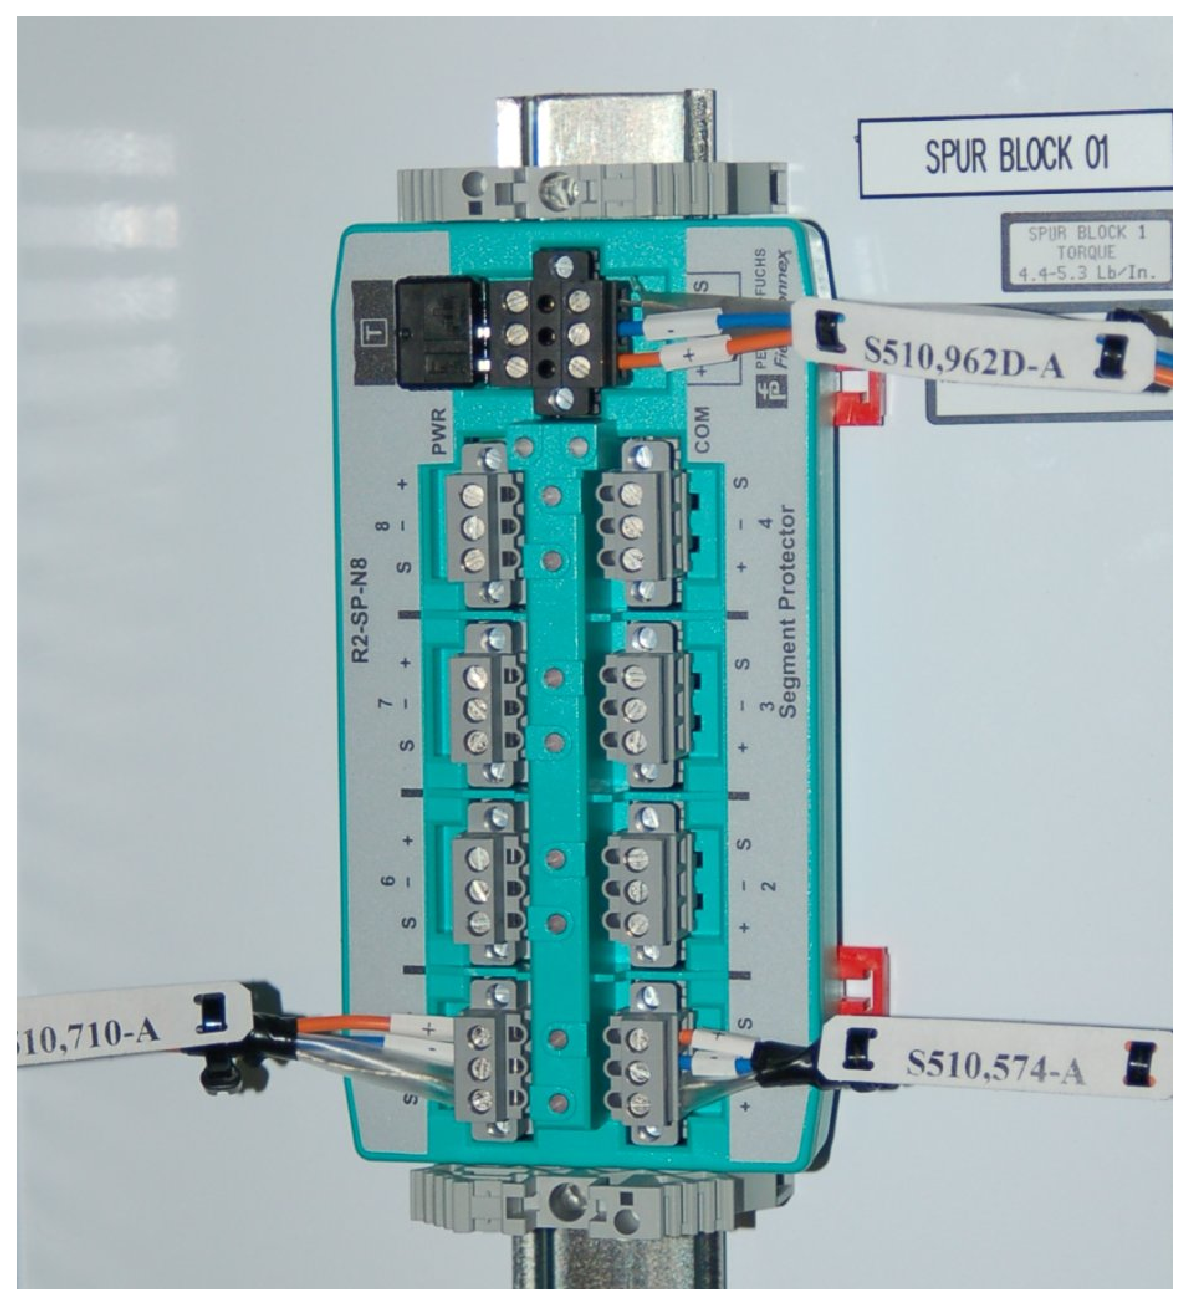
\includegraphics[width=4in]{fieldbus_39.eps}$$

This Fieldbus coupling device is aptly labeled a \textit{segment protector}, for it not only couples spurs to the main trunk of the Fieldbus segment, but it also guards against short-circuits in the spur cables and devices from interrupting communication on the rest of the segment.  If you look closely at the upper-left of the coupling device, you will see a black plastic square with two leads inserted into screw terminals: this is one of two \textit{terminating resistors} found in this Fieldbus segment, meaning this particular coupling device is at the ``end of the line'' of the network segment.

Not only do enclosure-protected coupling devices eliminate the need for special weather-proof connectors and instrument tray cable, but they also enjoy the radio interference immunity\footnote{Provided the metal enclosure's door is left in the closed position at all times!  Keying a radio transmitter near such a coupling device while the enclosure door is open invites trouble.} granted by being inside a metal cocoon.



\filbreak
\subsection{Electrical parameters}

FOUNDATION Fieldbus H1 networks use Manchester encoding to represent bit states: a ``high-to-low'' transition represents a logical zero (0), while a ``low-to-high'' transition represents a logical one (1).  The following illustration shows how the data stream \texttt{00100} would be represented in Manchester encoding:

$$\includegraphics{digital_07.eps}$$

FF devices must be able to correctly distinguish between rising- and fall-edge signals in order to properly interpret the bit states of a Manchester-encoded signal.  Any device interpreting these pulse edges ``backwards'' will invert every single bit!  Thankfully, this problem is easy to avoid because the DC power supplied by the H1 segment wiring provides a ``key'' to identifying which wire is which, and therefore which pulses are rising-edge versus which pulses are falling-edge.  For this reason, many (but not all!) FF devices are polarity-insensitive, automatically detecting the polarity of the network segment and compensating accordingly.

Every FF device draws at least 10 mA of current from the segment, and this current does not vary in the same manner that an analog (4-20 mA) device draws differing amounts of current under different operating conditions.  Always remember that a Fieldbus device signals its variable(s) digitally, not by varying current.  Old habits (and thought patterns) die hard, and so Fieldbus systems present challenges to technicians familiar with the behavior of analog current loop instrumentation.  The amount of current drawn by any particular FF device depends on that device's functionality -- obviously, some will require more current\footnote{Perusing documentation on an assortment of Emerson/Rosemount FF products, I found the following data: model 752 indicator = 17.5 mA, model 848L logic = 22 mA, model 848T temperature = 22 mA maximum, model 3244MV temperature = 17.5 mA typical, model DVC6000f valve positioner = 18 mA maximum, model 848L logic = 22 mA, model 848T temperature = 22 mA maximum, model 3244MV temperature = 17.5 mA typical, model 5500 guided-wave radar level = 21 mA, model 3095MV flow (differential pressure) = 17 mA approximate, model DVC6000f valve positioner = 18 mA maximum.} for their operation than others.  10 mA to 30 mA should be considered a general range of current drawn by each FF device.

The standard operating voltage range for FF devices is between 9 and 32 volts DC.  It is important to note, however, that not all manufacturers' devices are in full compliance with the Fieldbus Foundation standard, and as such some may not operate properly at low voltages (near 9 volts DC)!  The most common DC operating voltage for a FF network segment is 24 VDC (typical).

\vskip 10pt

The minimum transmission voltage of a FF device is 750 millivolts peak-to-peak, while the minimum signal level for reception by a FF device is 150 millivolts peak-to-peak.  This represents an acceptable attenuation of 5:1, or $-14$ dB between any two devices.






\filbreak
\subsection{Cable types}

Fieldbus cable is rated according to a four-level code (A, B, C, or D), each successive letter representing a cable of lower quality\footnote{I have successfully built several ``demonstration'' FF systems using cables of questionable quality, including lamp (``zip'') cord, with no termination resistors whatsoever!  If the distances involved are short, just about any cable type or condition will suffice.  When planning the installation of any real Fieldbus installation, however, you should never attempt to save money by purchasing lesser-grade cable.  The problems you will likely encounter as a consequence of using sub-standard cable will more than offset the initial cost saved by its purchase.}.  The following table gives \textit{minimum specifications} for each FF cable type:

% No blank lines allowed between lines of an \halign structure!
% I use comments (%) instead, so that TeX doesn't choke.

$$\vbox{\offinterlineskip
\halign{\strut
\vrule \quad\hfil # \ \hfil & 
\vrule \quad\hfil # \ \hfil & 
\vrule \quad\hfil # \ \hfil & 
\vrule \quad\hfil # \ \hfil & 
\vrule \quad\hfil # \ \hfil \vrule \cr
\noalign{\hrule}
%
% First row
\textbf{Cable Type} & \textbf{Type A} & \textbf{Type B} & \textbf{Type C} & \textbf{Type D} \cr
%
\noalign{\hrule}
%
% Another row
\textbf{Wire size} & AWG 18 & AWG 22 & AWG 26 & AWG 16 \cr
%
\noalign{\hrule}
%
% Another row
\textbf{Char. Impedance} & 100 $\Omega$ $\pm$ 20\% & 100 $\Omega$ $\pm$ 30\% & -- & -- \cr
%
\noalign{\hrule}
%
% Another row
\textbf{Shielding} & 1 for each pair & 1 for entire cable & none & none \cr
%
\noalign{\hrule}
%
% Another row
\textbf{Twisted pairs} & Yes & Yes & Yes & No \cr
%
\noalign{\hrule}
%
% Another row
\textbf{Max. length} & 1900 m & 1200 m & 400 m & 200 m \cr
%
\noalign{\hrule}
} % End of \halign 
}$$ % End of \vbox

Bear in mind that the maximum length given for each cable type is the \textit{total length} of all cables in a segment, trunk length plus all spur lengths.  As a general rule, spur lengths should be kept as short as possible.  It is better to route the trunk cable in a serpentine fashion to locate coupling devices close to their respective instruments than it is to streamline the trunk cable routing.  The following illustrations contrast the two approaches:

$$\includegraphics{fieldbus_11.eps}$$

$$\includegraphics{fieldbus_12.eps}$$

If greater lengths are required for a network segment, devices known as \textit{repeaters} may be added which sense and re-broadcast the Manchester-encoded FF signal between trunk cables.  A maximum of four repeaters may be used to extend any H1 segment.

\vskip 10pt

\filbreak

As always, neat wiring practices help make an instrument system easier to maintain and to diagnose when things go wrong.  The following photograph shows a triad of FOUNDATION Fieldbus junction boxes and (orange) network cables.  Coupling devices located inside each enclosure link each spur cable to the trunk:

$$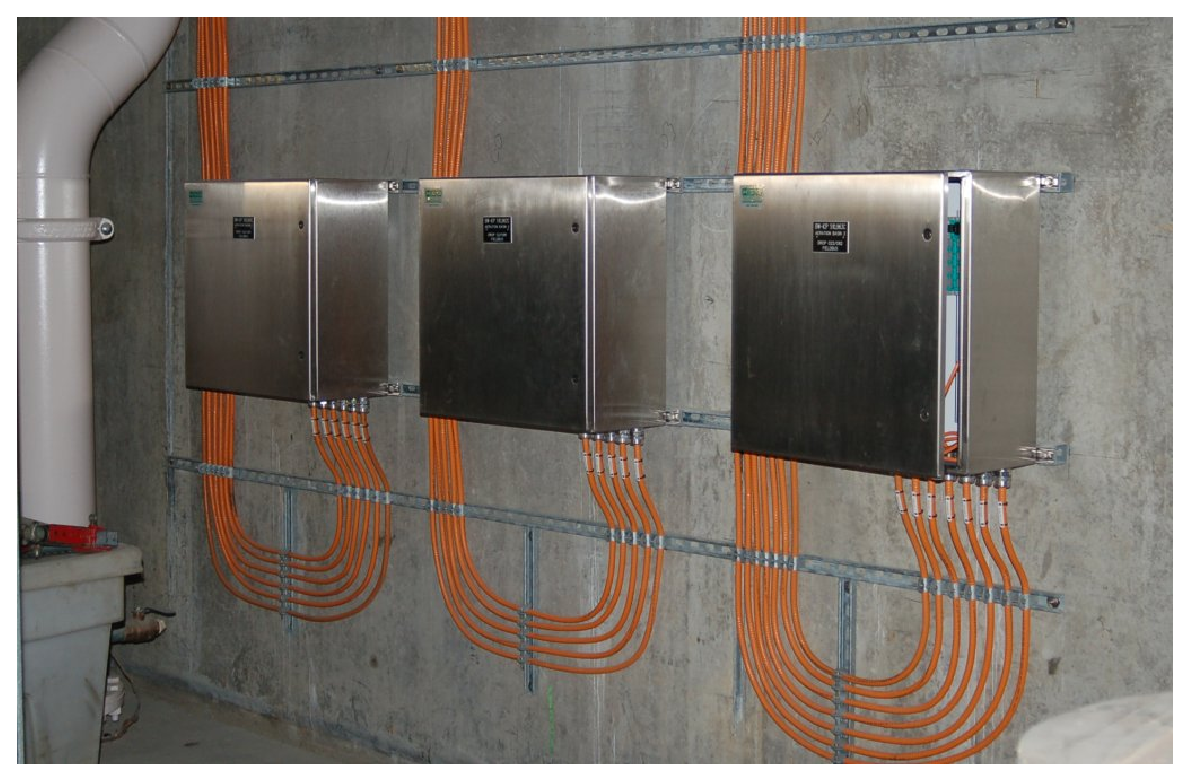
\includegraphics[width=5in]{fieldbus_40.eps}$$







\filbreak
\subsection{Segment design}

In addition to maximum (total) cable length and repeater count, a host of other details\footnote{Total device current draw, spur length versus number, intrinsic safety voltage and current limitations, etc.} conspire to limit how any particular H1 segment is wired.  To help engineers and technicians alike deal with these details, manufacturers often provide free \textit{segment design tool} software to pre-validate a segment design on computer before purchasing components and installing them in the field.  A screenshot taken from Emerson's offering shows what a typical FF segment layout might look like:

$$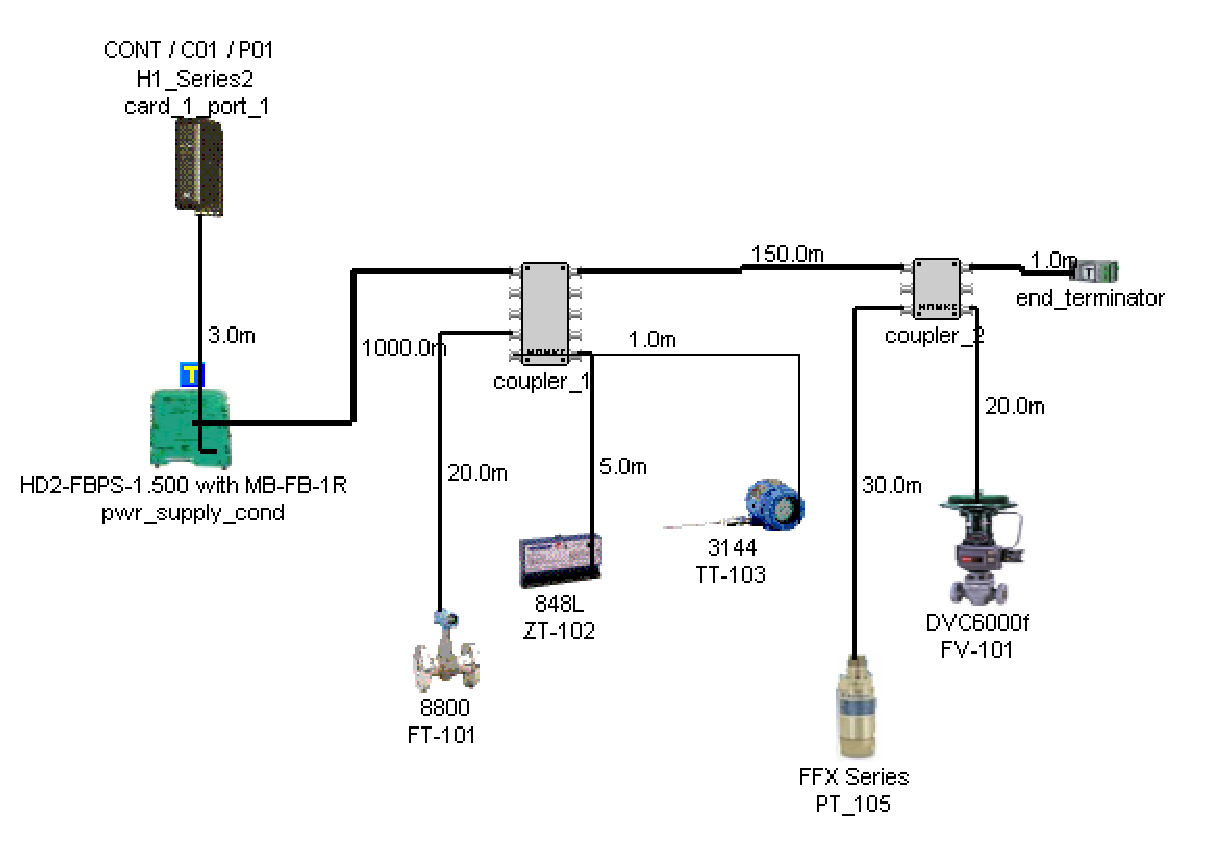
\includegraphics[width=6in]{fieldbus_10.eps}$$

A very nice feature of these segment design packages is their built-in database of FF components.  Every time you ``pick'' a particular component to place in your simulated segment, the program references data for that device's current draw and other electrical parameters relevant to the performance of the segment.  Of course, each manufacturer will tend to feature their own devices more prominently, and so these software tools sometimes feel like a promotional advertisement.  Despite the commercial aspect of their design, however, they are extremely useful in the planning stages of a FF network, and should be used whenever possible.

Another reason to use segment design tool software is to document the wiring of each FF segment.  One of the casualties of the new Fieldbus paradigm is the traditional \textit{loop diagram} (or ``loop sheet''), the purpose of which is to document the signal wiring dedicated for each measurement and control loop.  In FOUNDATION Fieldbus, the control ``loop'' is virtual rather than physical, being comprised of digital data sent between field instruments, the path of which being defined by the instruments' programming.  The only physical wiring entity to document in a FF system is the segment, and each segment most likely hosts more than one measurement and/or control loop.  Unless and until a standardized documentation format\footnote{At the time of this writing (2009), the ISA has yet to standardize new methods of FF documentation in the style of loop sheets and P\&IDs.  This is one of those circumstances where technology has outpaced convention.} is invented for Fieldbus network segments, the graphic image provided by segment design tool software is as good as anything.








\filbreak
\section{H1 FF Data Link layer}

Like so many other industrial data networks, FOUNDATION Fieldbus is an ``unswitched'' or ``broadcast'' type of network.  This means all data transmissions by all devices on a network are sensed by all the other devices.  In other words, there are no private messages between two devices on a shared network: every device ``hears'' every transmission from every other device.  This means devices must take turns communicating, with no simultaneous transmissions.  Layer 2 of the OSI Reference Model is where we define the ``data link'' elements of a digital data network, describing how individual devices negotiate for the right to transmit on the network.  Here is a list of some layer-2 properties of H1 FF networks:

\begin{itemize}
\item Master/slave network behavior for cyclic communications (i.e. one device polls the others, and the others merely respond)
\item Delegated token network behavior for acyclic communications (i.e. devices serially granted time to broadcast at will)
\item Dedicated  ``scheduler'' device for coordinating all segment communications
\item 8-bit address field (0 through 255 possible)
\item Maximum of 32 ``live'' devices on a segment
\end{itemize}

On an operating H1 segment, one device called the \textit{Link Active Scheduler} (abbreviated LAS) functions as the ``master'' device for coordinating all network communications, analogous to a police officer directing traffic in a road intersection.  The LAS device may be a regular field instrument (e.g. transmitter, valve positioner) or it may be the host system (i.e. the H1 segment interface card of a DCS).  The FF standard allows for one operating LAS device, with multiple back-up LAS devices waiting to take over if the primary LAS happens to fail for any reason.  

One of the tasks of the LAS is to ``compel'' the various field instruments to transmit their process control data (process variables, PID control output values, and other variables essential for loop monitoring and control), while the devices immediately respond in answer to the LAS's ``compel data'' command.  These critical communications occur on a regular schedule, and therefore are referred to as \textit{scheduled} or \textit{cyclic} communications.  Cyclic communication operates in a ``master-slave'' fashion, with the LAS acting as the master (commanding slave devices to broadcast specific data), and all other devices responding only when called upon by the LAS.  This form of communication is analogous to a traffic officer specifically directing one vehicle at a time to drive through an intersection in a prescribed manner.  \index{Cyclic communication, Fieldbus}  \index{Scheduled communication, Fieldbus}  \index{Link Active Scheduler}  \index{LAS}

Periods of time in between these critical transmissions on an H1 network are used for device's internal processing (e.g. PID algorithm execution, diagnostic checking) and also for less-critical data transmission.  It is during these \textit{unscheduled} or \textit{acyclic} times that devices are sequentially permitted (but not compelled) by the LAS to broadcast data of less importance such as operator setpoints, PID tuning constant updates, alarm acknowledgments, and diagnostic messages.  This form of communication is analogous to a traffic officer directing an entire lane of vehicles to enter the intersection at will.  \index{Acyclic communication, Fieldbus}  \index{Unscheduled communication, Fieldbus}

The scheduled nature of cyclic communication guarantees a certain maximum response time to critical control functions, an important property of control networks called \textit{determinism}.  Without determinism, a control system cannot be relied upon to perform critical regulatory functions in a timely\footnote{While many industrial control systems have been built using networks that are not strictly deterministic (e.g. Ethernet), generally good control behavior will result if the network latency time is arbitrarily short.  Lack of ``hard'' determinism is more of a problem in safety shutdown systems where the system \textit{must} respond within a certain amount of time in order to be effective in its safety function.  An industrial example of a safety system requiring ``hard'' determinism is compressor surge control.  An automotive example requiring ``hard'' determinism is anti-lock brake control.} manner, and sequencing\footnote{By ``sequencing,'' I mean the execution of all antecedent control functions prior to ``downstream'' functions requiring the processed data.  If in a chain of function blocks we have some blocks lagging in their execution, other blocks relying on the output signals of those lagging blocks will be functioning on ``old'' data.  This effectively adds dead time to the control system as a whole.  The more antecedent blocks in the chain that lag in time behind the needs of their consequent blocks, the more dead time will be present in the entire system.  To illustrate, if block \textit{A} feeds data into block \textit{B} which feeds data into block \textit{C}, but the blocks are executed in reverse order (C, then B, then A) on the same period, a lag time of \textit{three whole execution periods} will be manifest by the A-B-C algorithm.} of control functions such as PID, summers, subtractors, ratio multipliers, and the like may be compromised.  Thus, all the critical variables of a FF H1 loop are communicated between devices this way.  \index{Determinism, network}  \index{Hard determinism, network}  \index{Ethernet}








\filbreak
\subsection{Device addressing}

FOUNDATION Fieldbus devices (also called \textit{nodes}) are addressed by an eight-bit binary number when functioning on an H1 segment.  This binary number field naturally supports a maximum addressing range of 0 to 255 (decimal), or 00 to FF hexadecimal.  This address range is divided into the following sub-ranges by the Fieldbus Foundation:

% No blank lines allowed between lines of an \halign structure!
% I use comments (%) instead, so that TeX doesn't choke.

$$\vbox{\offinterlineskip
\halign{\strut
\vrule \quad\hfil # \ \hfil & 
\vrule \quad\hfil # \ \hfil & 
\vrule \quad\hfil # \ \hfil \vrule \cr
\noalign{\hrule}
%
% First row
\textbf{Address range} & \textbf{Address range} & \textbf{Allocation} \cr
(decimal) & (hexadecimal) &  \cr
%
\noalign{\hrule}
%
% Another row
0 through 15 & 00 through 0F & Reserved \cr
%
\noalign{\hrule}
%
% Another row
16 through 247 & 10 through F7 & Permanent devices \cr
%
\noalign{\hrule}
%
% Another row
248 through 251 & F8 through FB & New or decommissioned devices \cr
%
\noalign{\hrule}
%
% Another row
252 through 255 & FC through FF & Temporary (``visitor'') devices \cr
%
\noalign{\hrule}
} % End of \halign 
}$$ % End of \vbox

Devices are usually assigned addresses to function on the segment by the host system (typically a DCS with FF capability), although it is possible to order FF instruments pre-configured at the factory with addresses specified by the customer upon order.  Host systems are generally configured to automatically determine device addresses rather than require the technician or engineer to manually assign each address.  This makes the commissioning process more convenient.

The maximum number of ``permanent'' devices (installed field instruments) allowed on an H1 segment for operational reasons is 32, and as you can see the addressing scheme offers far more valid addresses than that.  One of the many tasks given to a segment's Link Active Scheduler (LAS) device is to probe for new devices connected to the segment.  This is done on a one-at-a-time basis, with the LAS sequentially polling for uncommissioned addresses within the valid address range.  Obviously, this can be a waste of time with only 32 addresses capable of active service at any given time and over 200 valid address numbers.  A practical solution to this problem is to specify an ``unused'' address range for the LAS to skip, so it does not waste time probing for devices (nodes) within a certain range.  This address range is specified as a set of two numbers: one for the First Unused Node (abbreviated \textit{FUN}), and another specifying the Number of Unused Nodes (abbreviated \textit{NUN}).  For example, if one wished to have the LAS on a particular H1 segment skip device addresses 40 through 211, one would configure the FUN to equal 40 and the NUN to equal 172, since the address range 40 through 211 is one hundred seventy two addresses (inclusive of both 40 and 211).  \index{FUN, Fieldbus addressing}  \index{NUN, Fieldbus addressing}

Even with a maximum operational limit of 32 devices to an H1 segment, it is rare to find segments operating with more than 16 devices.  One reason for this is speed: with additional devices requiring time to broadcast and process data, the total \textit{macrocycle} time (the time period between guaranteed delivery of the same process data from any one device -- the determinism time) must necessarily increase.  According to the Fieldbus Foundation's engineering recommendations guide, there must be no more than twelve devices on a segment (including no more than two final control elements) in order to achieve a 1-second or less macrocycle time.  For half-second update times, the recommended maximum is six devices (with no more than two final control elements).  For quarter-second update times, the limit drops to a total of three devices, with no more than one final control element.  Macrocycle time is essentially dead time, which is worse than lag time for any form of feedback control.  When controlling certain fast processes (such as liquid pressure or flow rate), dead times on the order of one second are a recipe for instability.  \index{Macrocycle}

Another limitation to the number of operational addresses on an H1 segment is current draw.  FF devices draw 10 mA of current \textit{minimum}.  A FF segment with sixteen parallel-connected devices would see a total current of 160 mA minimum, with a more realistic value being in excess of 300 mA.

\vskip 10pt

\filbreak

In addition to network addresses, each FF device bears an absolutely unique identifier (a 32-byte binary number) to distinguish it from any other FF device in existence.  This identifier serves much the same purpose as a \textit{MAC address} on an Ethernet device.  However, the identifier field for FF devices allows a far greater instrument count than Ethernet: 32 \textit{bytes} for FF instruments versus 48 bits for Ethernet devices.  While the Ethernet MAC address field only allows for a paltry $2.815 \times 10^{14}$ unique devices, the FF identifier allows $1.158 \times 10^{77}$ devices!  The distinction between a FF device's network address and the device's identifier is virtually identical to the distinction between an Ethernet device's IP address assigned by the end-user and its MAC address number assigned by the manufacturer.   \index{MAC address, Ethernet}  \index{Identifier, Fieldbus device}  \index{Ethernet}

This identifier value is usually expressed as 32 ASCII-encoded characters for brevity (one alphanumeric character per byte), and is subdivided into byte groups as follows:

% No blank lines allowed between lines of an \halign structure!
% I use comments (%) instead, so that TeX doesn't choke.

$$\vbox{\offinterlineskip
\halign{\strut
\vrule \quad\hfil # \ \hfil & 
\vrule \quad\hfil # \ \hfil & 
\vrule \quad\hfil # \ \hfil \vrule \cr
\noalign{\hrule}
%
% First row
\textbf{First 6 bytes} & \textbf{Middle 4 bytes} & \textbf{Last 22 bytes} \cr
%
\noalign{\hrule}
%
% Another row
Manufacturer code & Device type code & Serial number \cr
%
\noalign{\hrule}
} % End of \halign 
}$$ % End of \vbox

For example, the identifiers for all \textit{Fisher} brand devices begin with the first six characters \texttt{005100}.  The identifiers for all \textit{Smar} devices begin with the characters \texttt{000302}.  The identifiers for all \textit{Rosemount}\footnote{The engineers there are not without a sense of humor, choosing for their manufacturer code the same model number as the venerable model 1151 differential pressure transmitter, perhaps the most popular Rosemount industrial instrument in the company's history!} brand devices begin with \texttt{001151}.  A typical identifier (this particular one for a Fisher model DVC5000f valve positioner) appears here:

$$\hbox{\texttt{005100 0100 FISHERDVC0440761498160}}$$

Normally, these identifiers appear as 32-character strings, without spaces at all.  I have inserted spaces within this string to make the character groupings easier to see.








\filbreak
\subsection{Communication management}

In a FF network segment, the Link Active Scheduler (LAS) device coordinates all communications between segment devices.  Among the many responsibilities the LAS is tasked with are the following:

\begin{itemize}
\item Commands non-LAS devices to broadcast data to the segment with ``Compel Data'' (CD) messages, issued at regular time intervals to specific devices (one at a time)
\item Permits non-LAS devices to voluntarily communicate with ``Pass Token'' (PT) messages, issued during unscheduled time slots to specific devices (one at a time, in ascending order of address number)
\item Keeps all segment devices synchronized with a regular ``Time Distribution'' (TD) message
\item Probes for new devices on the segment with a ``Probe Node'' (PN) message
\item Maintains and publishes a list of all active devices on the network (the \textit{Live List})
\end{itemize}




\filbreak
\subsubsection{Scheduled versus unscheduled communication}

As previously mentioned, Fieldbus H1 network communication may be divided into two broad categories: \textit{scheduled} (cyclic) and \textit{unscheduled} (acyclic).  Scheduled communication events are reserved for exchanging critical control data such as process variable measurements, cascaded setpoints, and valve position commands.  These scheduled communications happen on a regular, timed schedule so that loop determinism is guaranteed.  Unscheduled communications, by contrast, are the way in which all other data is communicated along an H1 segment.  Manual setpoint changes, configuration updates, alarms, and other data transfers of lesser importance are exchanged between devices in the times between scheduled communication events.  \index{Cyclic communication, Fieldbus}  \index{Scheduled communication, Fieldbus}  \index{Acyclic communication, Fieldbus}  \index{Unscheduled communication, Fieldbus}

Both forms of communication are orchestrated by the Link Active Scheduler (LAS) device, of which there is only one active at any given time\footnote{In addition to the main LAS, there may be ``backup'' LAS devices waiting ready to take over in the event the main LAS fails for any reason.  These are Link Master devices configured to act as redundant Link Active Schedulers should the need arise.  However, at any given time there will be only \textit{one} LAS.  In the event of an LAS device failure, the Link Master device with the lowest-number address will ``step up'' to become the new LAS.} on an H1 segment.  The LAS issues ``token'' messages to non-LAS devices commanding (or merely authorizing) them to broadcast to the segment one at a time.  Each token message issued by the LAS confers transmission rights to an FF device either for a limited purpose (i.e. the precise message to be transmitted) or for a limited time (i.e. giving that device the freedom to transmit whatever data it desires for a short duration), after which transmission rights return to the LAS.  

CD tokens are both compulsory and message-specific: each one issued by the LAS commands a single device to immediately respond with a broadcast of some specific data.  This is how scheduled (cyclic) communication is managed, intended for the deterministic communication of critical data necessary for automatic process control functions.  By contrast, PT tokens are both voluntary and time-specific: each one issued by the LAS grants a single device free time to transmit data of lesser importance.  This is how unscheduled (acyclic) communication between devices is managed, intended for the non-deterministic communication of status messages and human interactions with the control system (e.g. mode changes, maintenance, alarms, parameter adjustments).   \index{Compel Data (CD) token, Fieldbus}   \index{Pass Token (PT), Fieldbus}

The LAS also issues a third type of token message: the ``Probe Node'' (PN) token intended to elicit a response from any new devices connected to the network segment.  Probe Node tokens are issued one at a time to each uncommitted device address in search of any new devices.  \index{Probe Node (PN) token, Fieldbus}

In addition to transmitting tokens -- which by definition are messages granting another device permission to transmit to the network -- the LAS also broadcasts other messages necessary for the function of an H1 segment.  For example, the ``Time Distribution'' (TD) message regularly broadcast by the LAS keeps all devices' internal clocks synchronized, which is important for the coordinated transfer of data.  \index{Time Distribution (TD) message, Fieldbus}

One of the ``internal'' tasks of the LAS not requiring network broadcasts is the maintenance of the \textit{Live List}, which is a list of all known devices functioning on the network segment.  New devices responding to ``Probe Node'' messages will be added to the Live List when detected.  Devices failing to return or use PT tokens issued to them are removed from the Live List after a number of attempts.  When ``backup'' LAS devices exist on the segment, the LAS also publishes updated copies of the Live List to them, so they will have the most up-to-date version should the need arise to take over for the original LAS (in the event of an LAS device failure).  \index{Live List, Fieldbus}

\vskip 10pt

\filbreak

In ``busy'' H1 segments where multiple devices are exchanging data with each other, a heavy traffic load of scheduled communications (CD tokens and their responses) makes it difficult for substantial unscheduled (acyclic) data exchanges to occur.  For example, if a device happens to be maintaining a lengthy list of client/server requests in its queue, which it may address only during its allotted acyclic time slots (i.e. when it has been given the PT token from the LAS), it is quite possible the PT token will expire before all the device's transactions have been completed.  This means the device will have to wait for the next acyclic period before it can complete all the unscheduled communication tasks in its queue.  The Fieldbus Foundation recommends new H1 segments be configured for no more than 30\% scheduled communications during each macrocycle (70\% unscheduled time).  This should leave plenty of ``free time'' for all necessary acyclic communications to take place without having to routinely wait multiple macrocycles.





\filbreak
\subsubsection{Virtual Communication Relationships}

A term you will frequently encounter in FF literature is \textit{VCR}, or ``Virtual Communication Relationship.''  There are three different types of VCRs in FF, describing three different ways in which data is communicated between FF devices:  \index{VCR, Fieldbus}  \index{Virtual Communication Relationship (VCR), Fieldbus}

\begin{itemize}
\item \textbf{Publisher/Subscriber} (scheduled), otherwise known as Buffered Network-scheduled Unidirectional (BNU)
\item \textbf{Client/Server} (unscheduled), otherwise known as Queued User-triggered Bidirectional (QUB)
\item \textbf{Source/Sink} (unscheduled), otherwise known as Queued User-triggered Unidirectional (QUU)
\end{itemize}  \index{BNU, Fieldbus}  \index{QUB, Fieldbus}  \index{QUU, Fieldbus}  

\vskip 10pt

\noindent
\underbar{Publisher/Subscriber}: this VCR describes the action of a Compel Data (CD) token.  The Link Active Scheduler (LAS) calls upon a specific device on the network to transmit specific data for a time-critical control purpose.  When the addressed device responds with its data, multiple devices on the network ``subscribing'' to this published data receive it simultaneously.  This is how process-control variables (PV, PID output, etc.) are communicated between instruments comprising a FF control loop.  The publisher/subscriber VCR model is highly deterministic because all such communications occur on a precisely defined schedule.

\vskip 10pt

\noindent
\underbar{Client/Server}: this VCR describes one class of unscheduled communications, permitted when a device receives a Pass Token (PT) message from the LAS.  Each device maintains a queue (list) of data requests issued by other devices (clients), and responds to them in order as soon as it receives the Pass Token.  By responding to client requests, the device acts as a server.  Likewise, each device can use this time to act as a client, posting their own requests to other devices, which will act as servers when they receive the PT token from the LAS.  This is how non-critical messages such as maintenance and device configuration data, operator setpoint changes, alarm acknowledgments, PID tuning values, etc. are exchanged between devices on an H1 segment.  Trend data (process variables recorded over time and displayed in time-domain graph form) may also be communicated using this type of VCR, with a ``burst'' of collected samples communicated per server message\footnote{The Source/Sink VCR is the preferred method for communicating trend data, but trends may be communicated via any of the three VCR types.  All other factors being equal, acyclic communication (either Source/Sink or Client/Server) of trend data occupies less network bandwidth than cyclic communication (Publisher/Subscriber).}.  Client/server communications are checked for data corruption by their receivers, to ensure reliable data flow.

\vskip 10pt

\noindent
\underbar{Source/Sink} (also called \underbar{Report Distribution}): this VCR describes another class of unscheduled communications, permitted when a device receives a Pass Token (PT) message from the LAS.  This is where a device broadcasts data out to a ``group address'' representing many devices.  Source/sink communications are not checked for data corruption, as are client/server communications.  Examples of messages communicated in a FF segment using the source/sink VCR include trend reports and alarms.

\vskip 10pt

An analogy for making sense of VCRs is to imagine lines drawn between FF devices on a segment to connect their various messages to other devices.  Each line represents an individual transmission which must take place some time during the macrocycle.  Each line is a VCR, some managed differently than others, some more critical than others, but all of them are simply communication events in time.  A specific example of this is in the function block diagrams for a FF control system, where connecting lines between function blocks residing in different devices represent messages sent by the Publisher/Subscriber VCR method.  Each line connecting function blocks between different devices is a message in response to a CD (Compel Data) token issued by the LAS, ensuring the deterministic transfer of critical control data between function blocks necessary for the control system to reliably function.

\filbreak

For example, consider this H1 segment connected to an interface card on a DCS rack, followed by a P\&ID showing the relationships between the instruments:

$$\includegraphics{fieldbus_35.eps}$$

Loop 211 is a simple PID level control, regulating liquid level in the reactor vessel by releasing liquid from the bottom.  Loop 187 is a simple indicating/recording system for temperature and flow, the signals coming from a multivariable transmitter.  Loop 231 is a cascaded pressure/flow control system, with reactor pressure as the master variable and feed flow as the slave variable: the pressure controller (residing inside pressure transmitter PT-231) provides remote setpoint values to the flow controller (residing in the flow control valve FV-231), which then adjusts the position of the valve to achieve the desired feed flow rate into the reactor until reactor pressure stabilizes at setpoint.

Note the different line types used to represent digital signals in the P\&ID: lines with diamond symbols represent data sent over Fieldbus cable, while lines with hollow circles represent data sent between functions within the same physical device.  These latter ``internal'' data links help the reader discern which functions reside in which physical instruments.  Functions residing within the same FF device must also share the same loop number.  These standards for P\&ID notation come from the Fieldbus Foundation's \textit{System Engineering Guidelines} document (revision 2.0, page 72) and from the ANSI/ISA-5.1-2009 ``Instrumentation Symbols and Identification'' standard.

For example, the PID control function represented by FC-231 resides within the valve positioner (FV-231), because those two bubbles share the same loop number and are connected with lines having hollow circles (which means they are parts of one homogeneous system rather than independent instruments).  Likewise, the same line symbology tells us that pressure control PID function PC-231 resides within the pressure transmitter PT-231.

\filbreak

Control-critical variables communicated over the segment between devices include the output value of PC-231 (cascade flow controller FC-231's remote setpoint value), flow transmitter FT-231's process variable measurement, and the process variable from level transmitter LT-211.  These are all Publisher/Subscriber VCRs, transmitted at the request of a Compel Data (CD) token issued by the LAS device on a tightly controlled schedule.  PC-231, FT-231, and LT-211 \textit{publish} their data to the H1 segment one at a time (each broadcast at the command of a separate CD token issued by the LAS), with FC-231 \textit{subscribing} to PC-231's and FT-231's data, and LC-211 \textit{subscribing} to LT-211's data:  \index{Back-calculation variable, FOUNDATION Fieldbus function block programming}

$$\includegraphics{fieldbus_36.eps}$$

\filbreak

Messages such as operator-adjusted setpoint values and maintenance tasks occur as Client/Server VCRs, done during the ``unscheduled'' communication times in the LAS's sequence.  The LAS device issues Pass Token (PT) messages to each device, giving permission for each device (one at a time) to transmit such information as necessary.  Examples of such non-critical messages in our reactor control system are shown here:

$$\includegraphics{fieldbus_37.eps}$$

In this example, LC-211 is a \textit{client} to the operator's display console which \textit{serves} setpoint and tuning parameter data to that controller.  Likewise, PC-231 is a \textit{client} receiving setpoint data \textit{served} by the operator console.  FT-187 is a \textit{client} to either a portable Fieldbus communication device or to an engineering workstation in the control system where a technician \textit{serves} new process variable range parameters to it.

\filbreak

Finally, our third VCR (Source/Sink) finds application in the reactor control system for flow transmitter FT-187, broadcasting its flow trend data during ``unscheduled'' periods in the LAS's cycle, as well as for instrument alarm messages.  Like the Client/Server messages, this one is prompted when the device receives a special Pass Token (PT) signal from the LAS, giving temporary permission for that device to broadcast its data:

$$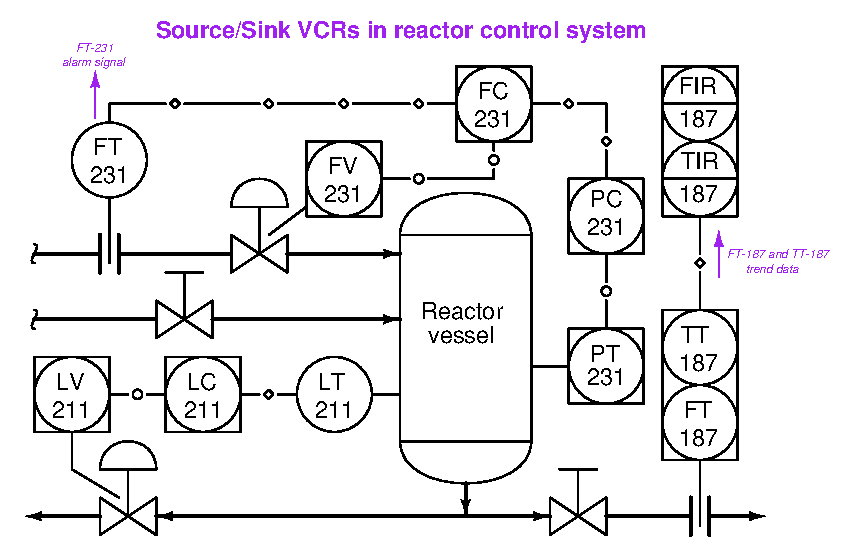
\includegraphics{fieldbus_38.eps}$$

In this example, we see FT-231 \textit{sourcing} an alarm message to an operator console which functions as a \textit{sink} for that data.  Likewise, TT-187 and FT-187 both \textit{source} trend data while TIR-187 and FIR-187 \textit{sink} that data, respectively.








\filbreak
\subsection{Device capability}

Not all FF devices are equally capable in terms of Data Link (layer 2) functions.  The FF standard divides data link device functionality into three distinct groups, shown here in order of increasing capability:

\begin{itemize}
\item Basic devices
\item Link Master devices
\item Bridge devices
\end{itemize}

A \textit{Basic} device is one capable of receiving and responding to tokens issued by the Link Active Scheduler (LAS) device.  As discussed previously, these tokens may take the form of Compel Data (CD) messages which command immediate response from the Basic device, or Pass Token (PT) messages which grant the Basic device time-limited access to the segment for use in broadcasting data of lesser importance.

A \textit{Link Master} device is one with the ability to be configured as the LAS for a segment.  Not all FF devices have this ability, due to limited processing capability, memory, or both\footnote{Some FF devices capable of performing advanced function block algorithms for certain process control schemes may have the raw computational power to be an LAS, but the manufacturer has decided not to make them Link Master capable simply to allow their computational power to be devoted to the function block processing rather than split between function block tasks and LAS tasks.}.

A \textit{Bridge} device links multiple H1 segments together to form a larger network.  Field instruments are never Bridge devices -- a Bridge is a special-purpose device built for the express purpose of joining two or more H1 network segments.















\filbreak
\section{FF function blocks}

Data-processing modules within FF systems are known as \textit{function blocks}.  Sometimes these blocks serve merely to catalogue data, while in other instances the blocks execute specific algorithms useful for process measurement and control.  These ``blocks'' are not physical entities, but rather abstract software objects -- they exist only as bits of data and instructions in computer memory.  However, the blocks are represented on FF computer configuration displays as rectangular objects with input ports on the left-hand side and output ports on the right-hand side.  The construction of a working control system comprised of FF devices consists of linking the outputs of certain function blocks with the inputs of other function blocks via configuration software and computer-based tools.  This usually takes the form of using a computer to draw connecting lines between the output and input ports of different function blocks.




\filbreak
\subsection{Analog function blocks versus digital function blocks}

Function-block programming in general strongly resembles the design philosophy of legacy analog-based computer systems, where specific functions (addition, subtraction, multiplication, ratio, time-integration, limiting, and others) were encapsulated in discrete operational amplifier circuits, and whole systems were built by connecting function blocks together in whatever patterns were desired to achieve a design goal.  Here with Fieldbus programming, the function blocks are virtual (bits and data structures in digital memory) rather than real analog circuits, and the connections between blocks are merely pointer assignments in digital memory rather than actual ``patch cable'' connections between circuit boards.

\filbreak

An example contrasting analog circuit design with Fieldbus function-block design appears here, both systems selecting the \textit{greatest} temperature signal to be the output.  The system on the left-hand side receives analog voltage signals from three temperature sensors, using a network of operational amplifiers, diodes, and resistors to select the greatest voltage signal to be the output.  The system on the right-hand side uses three Fieldbus transmitters to sense temperature, the greatest temperature signal selected by an algorithm (the ISEL function block) running in a Fieldbus device.  The device running the ISEL function could be one of the three FF temperature transmitters, or another device on the segment:

$$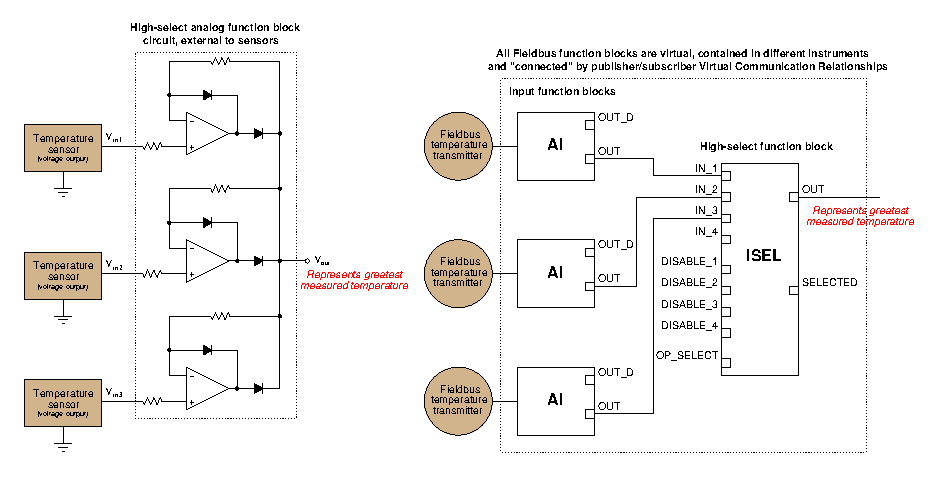
\includegraphics{fieldbus_22.eps}$$

Instead of analog voltage signals sent by wire to special-function circuit modules, FOUNDATION Fieldbus uses digital messages sent over an H1 network segment to special-function software ``blocks'' running inside ordinary Fieldbus devices.  The lines connecting different function blocks together in a FOUNDATION Fieldbus system show the sources and destinations of these digital messages.  If two FF function blocks reside in different FF devices, the connecting lines represent publisher/subscriber communication assignments coordinated by the Link Active Scheduler (LAS) device.





\filbreak
\subsection{Function block location}

There is usually some freedom of choice in where various function blocks may be located in a FF segment.  Take for example the following flow control loop, where a flow transmitter feeds measured flow data into a PID control function block, which then drives a control valve to whatever position necessary to regulate flow.  The actual physical device layout might look something like this:

$$\includegraphics[width=6in]{fieldbus_23.eps}$$

The function block connections necessary for this control scheme to work are shown in the next diagram, coupling the AI (analog input) block located in the transmitter to a PID control block to an AO (analog output) block located in the valve positioner:

$$\includegraphics{fieldbus_24.eps}$$

All function block inputs are on the left-hand sides of the blocks, and all outputs are on the right-hand sides.  In this function block program, data from the analog input (AI) block flows into the PID block.  After calculating the proper output value, the PID block sends data to the analog output (AO) block where the final control element (e.g. valve, variable-speed motor) is adjusted.  The AO block in turn sends a ``back calculation'' signal to the PID block to let it know the final control element has successfully reached the state commanded by the PID block's output.  This is important for the elimination of \textit{reset windup}\footnote{``Reset windup'' which is also known as ``integral windup'' is what happens when any loop controller possessing reset (integral) action senses a difference between PV and SP that it cannot eliminate.  The reset action over time will drive the controller's output to saturation.  If the source of the problem is a control valve that cannot attain the desired position, the controller will ``wind up'' or ``wind down'' in a futile attempt to drive the valve to a position it cannot go.  In an FF system where the final control element provides ``back calculation'' feedback to the PID algorithm, the controller will not attempt to drive the valve farther than it is able to respond.} in the event the final control element fails to respond to the PID block's output signal.  \index{Back-calculation variable, FOUNDATION Fieldbus function block programming} 

It should be obvious that the analog input (AI) block must reside in the transmitter, simply because only the transmitter is able to measure the process fluid flow rate.  Likewise, it should be obvious that the analog output (AO) block must reside in the control valve positioner, simply because the valve is the only device capable of manipulating (exerting influence over) anything.  However, given the lack of a separate controller device, the person configuring the Fieldbus loop may choose to locate the PID block in either the transmitter or the control valve positioner.  So long as both the FF transmitter and the FF valve positioner possess PID function block capability, it is possible to locate the PID function block in either device.

\filbreak

The following illustrations show the two possible locations of the PID function block in this system:

$$\includegraphics{fieldbus_25.eps}$$

The only factor favoring one location over another for the PID function block is the number of communication broadcasts (``Compel Data'' token distributions and replies) necessary per macrocycle.  Note the lines connecting function blocks between the two instruments in the previous diagrams (lines crossing from one blue bubble to another).  Each of these lines represents a VCR (Virtual Communication Relationship) -- an instance during each macrocycle where data must be transmitted over the network segment from one device to another.  With the PID function block located in the flow transmitter, two lines connect blocks located in different physical devices.  With the PID function block located in the valve positioner, only one line connects blocks in different physical devices.  Thus, locating the PID function block in the valve positioner means only one CD message/reply is necessary per macrocycle, making the network communication more efficient.

\filbreak

To illustrate the difference this re-location of the PID block makes, we will examine the function block diagram and macrocycle timing schedule on a simple pressure control FF loop, hosted on an Emerson DeltaV distributed control system.  The first composite screenshot shows the function block diagram and schedule with the PID function block located in the transmitter (PT\_501):

$$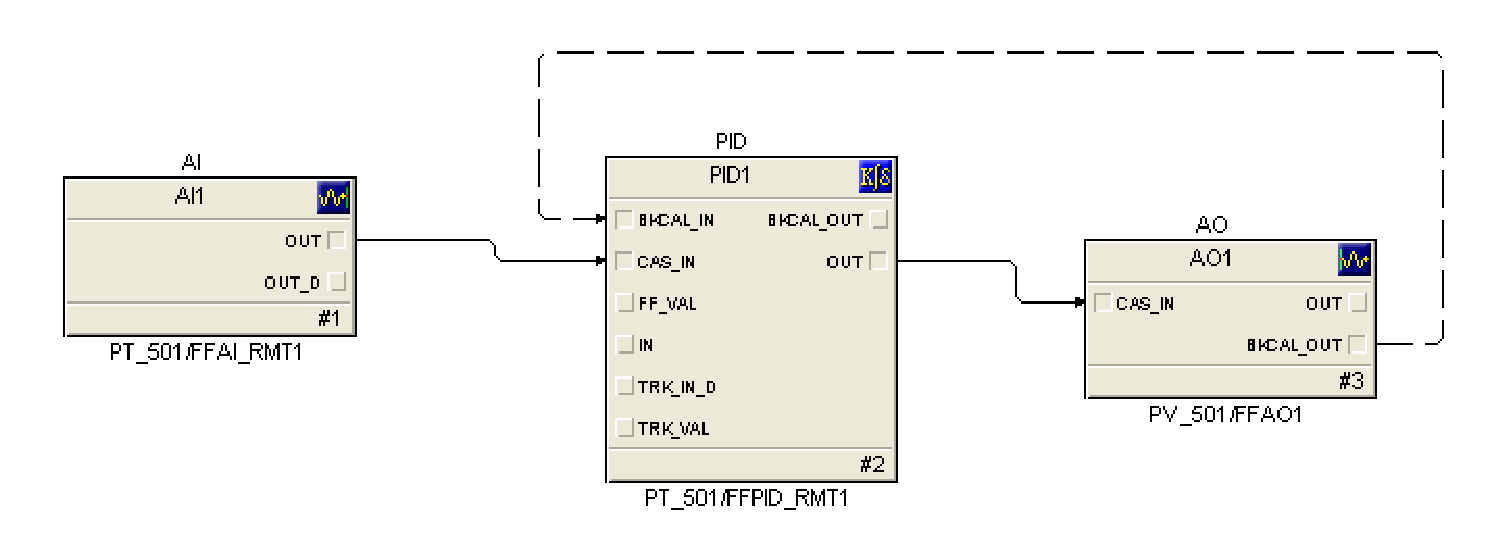
\includegraphics[width=4in]{fieldbus_26.eps}$$

$$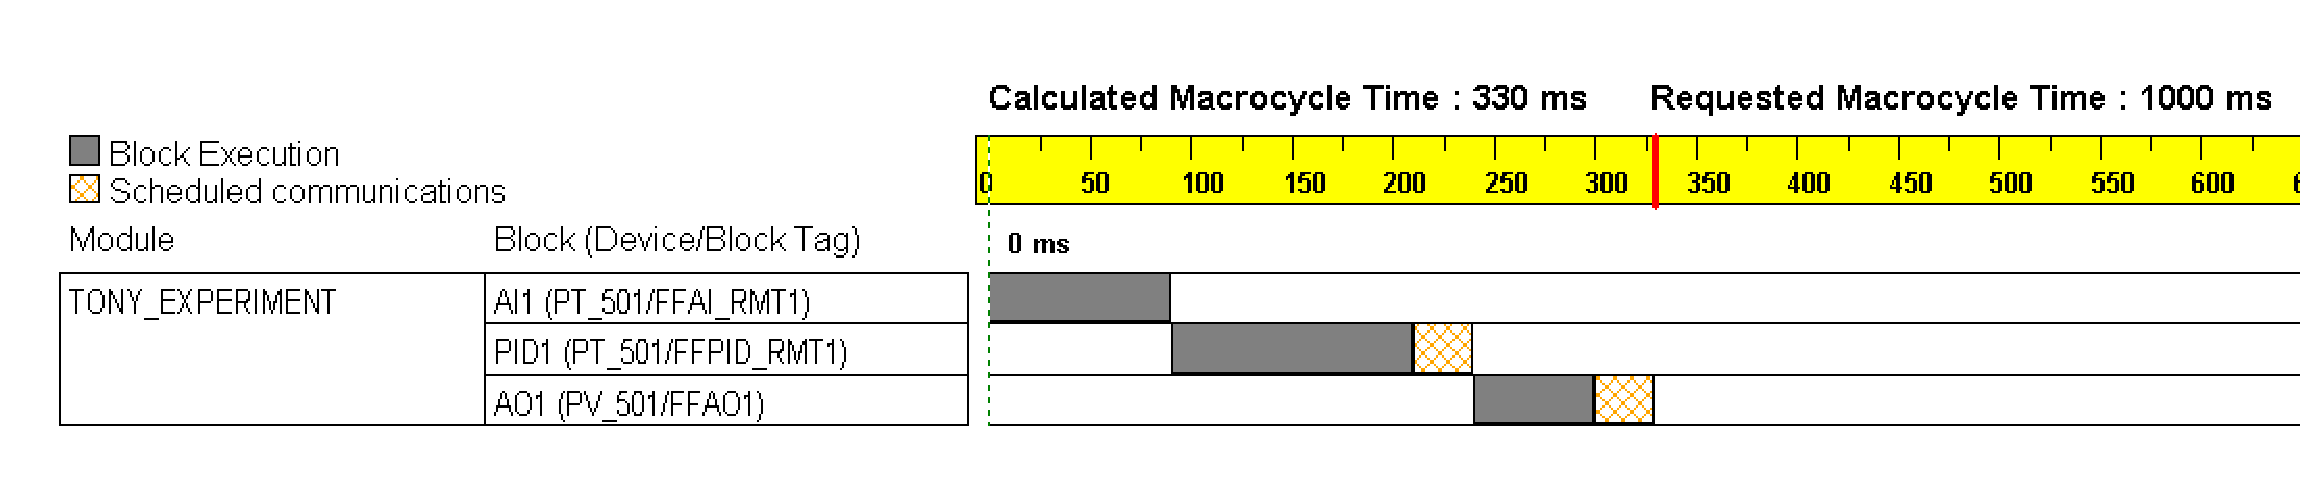
\includegraphics[width=6in]{fieldbus_27.eps}$$

Note the two scheduled communication events (CD tokens and responses) necessary in the macrocycle schedule to enable communication between pressure transmitter PT\_501's PID function block and valve positioner PV\_501's analog output function block.  The first CD token in this macrocycle schedule compels the PID block to publish its ``output'' signal (subscribed to by the analog output block), while the second token compels the analog output block to publish its ``back calculation'' signal (subscribed to by the PID block).  The amount of time required for function block execution and their publisher/subscriber communications is 330 milliseconds, with a total macrocycle time of 1 second\footnote{This is not an unreasonable loop execution time for a gas pressure control system.  However, \textit{liquid} pressure control is notoriously fast-acting, and will experience less than ideal response with a controller dead time of one second.}.

\filbreak

Now let's examine the same PID pressure control system with the PID function block moved to the valve.  Here you see the function block diagram followed immediately by the updated macrocycle schedule:

$$\includegraphics[width=4in]{fieldbus_28.eps}$$

$$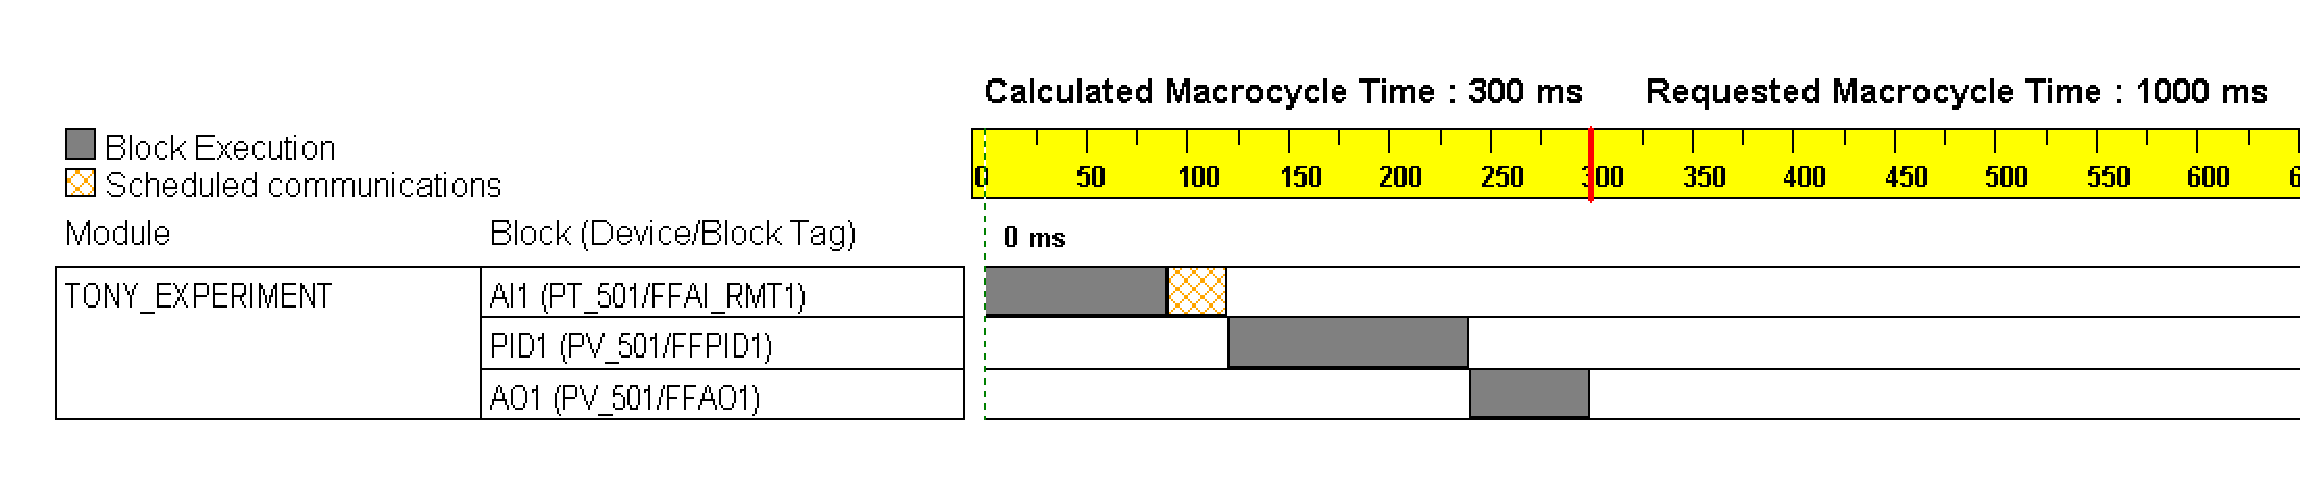
\includegraphics[width=6in]{fieldbus_29.eps}$$

In this macrocycle timing schedule, there is only one CD token needed: compelling the analog input block to publish its measurement signal (subscribed to by the PID block).  This makes the block execution plus scheduled communication time 30 milliseconds shorter than before (300 milliseconds total as opposed to 330 milliseconds), since there is one less scheduled communications event happening.  The total macrocycle time of 1 second remains unchanged, but now we have 30 milliseconds more unscheduled time during which other communication events may take place.






\filbreak
\subsection{Standard function blocks}

The FF standard specifies many different function blocks for the construction of control algorithms.  Ten of them are considered ``basic'' FF function blocks:

\begin{itemize}
\item \texttt{AI} -- Analog Input
\item \texttt{AO} -- Analog Output
\item \texttt{B} -- Bias
\item \texttt{CS} -- Control Selector
\item \texttt{DI} -- Discrete Input
\item \texttt{DO} -- Discrete Output
\item \texttt{ML} -- Manual Loader
\item \texttt{PD} -- Proportional/Derivative control
\item \texttt{PID} -- Proportional/Integral/Derivative control
\item \texttt{RA} -- Ratio
\end{itemize}

\vskip 10pt

Nineteen more ``Advanced'' function blocks are incorporated in the FF standard:

\begin{itemize}
\item Pulse Input
\item Complex Analog Output
\item Complex Discrete Output
\item Step Output PID
\item Device Control
\item Setpoint Ramp
\item Splitter
\item Input Selector
\item Signal Characterizer
\item Dead Time
\item Calculate
\item Lead/Lag
\item Arithmetic
\item Integrator
\item Timer
\item Analog Alarm
\item Discrete Alarm
\item Analog Human Interface
\item Discrete Human Interface
\end{itemize}

\vskip 10pt

Five more function blocks are specified as well:

\begin{itemize}
\item Multiple Analog Input
\item Multiple Analog Output
\item Multiple Digital Input
\item Multiple Digital Output
\item Flexible Function Block
\end{itemize}

The primary benefit of standardization is that the end-user may choose FF instruments manufactured by any standard-compliant vendor, and those function blocks should behave the same as the equivalent function blocks within any other manufacturer's model of FF device.  There are, of course, examples where manufacturers have equipped their FF devices with ``extended'' capability function blocks going beyond the Fieldbus Foundation standard, and the user must beware of this.






\filbreak
\subsection{Device-specific function blocks}

In addition to the function blocks necessary to construct control schemes, all FF instruments contain one \textit{Resource} block and usually one or more \textit{Transducer} blocks describing details specific to that instrument.  The following computer screenshot shows all function blocks within a Rosemount model 3095MV Fieldbus transmitter:  \index{Rosemount model 3095MV multi-variable transmitter}  \index{Resource block, Fieldbus}  \index{Transducer block, Fieldbus}

$$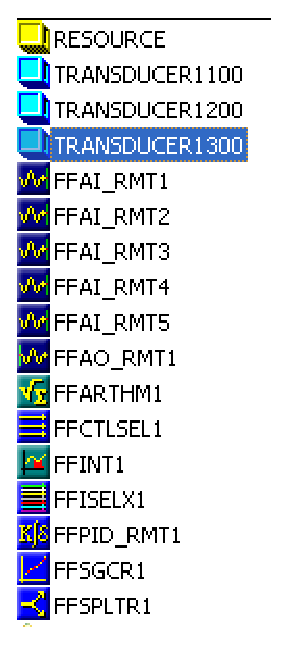
\includegraphics[height=2.5in]{fieldbus_21.eps}$$  % This graphic is 405 pixels wide and 580 pixels tall

The Resource block appears first in this list, followed by three transducer blocks, then followed by the palette of general function blocks for use in constructing control algorithms.  Information contained in the Resource block of an FF instrument includes the following:

\begin{itemize}
\item Identifier (the 32-byte code unique to every FF device)
\item Type of device
\item Device revision level
\item Memory total and available (free) capacity
\item Computation time
\item Available features listing
\item Current device state (Initializing, Standby, On-line, Failed, etc.)
\end{itemize}

Transducer blocks provide a means of organizing data relevant to the actual sensing inputs, outputs, calculated variables, and graphic displays of a FF device.  There need not be a one-to-one correspondence between the number of transducer blocks in an FF device and the number of physical I/O channels it has.  For example, in the Rosemount 3095MV multivariable transmitter, transducer block 1100 manages all physical measurement inputs (pressure and temperature sensors) while transducer block 1200 is reserved for inferred mass flow (based on calculations performed on the raw sensor measurements) and transducer block 1300 manages data for the liquid crystal display (LCD).  \index{Inferred variable}







\filbreak
\subsection{FF signal status}

As mentioned earlier, function block programming bears a strong resemblance to analog function-block circuit design, where specific tasks are divided up into discrete elements, those elements connected together to form a larger system with more complex functionality.  One of the important distinctions between legacy analog function block circuit design and FF function block programming is the data content of the lines connecting blocks together.  In the analog world, each connecting line (wire) carries exactly one piece of information: a single variable represented in analog form by a voltage signal.  In the world of Fieldbus, each connecting line carries not only the variable's numerical value, but also a \textit{status} and in some cases an \textit{engineering unit} (a unit of measurement).  For example, a Fieldbus transmitter sensing temperature might output a digital process variable (PV) signal of ``342 degrees Celsius, Good'', whereas a temperature transmitter with an analog (e.g. 4-20 mA) output is merely able to send a signal representing the temperature (no measurement unit or status information).

The inclusion of status along with data is a powerful concept, with roots in scientific practice.  Scientists, as a rule, do their best to report the degree of \textit{confidence} associated with the data they publish from experiments.  Data is important, of course, but so is the degree of certainty with which that data was obtained.  Obviously, data gathered with instruments of low quality (high uncertainty) will have different significance than data gathered with instruments of high precision and impeccable accuracy (low uncertainty).  Any scientist basing research on a set of scientific data published by another scientist will have access to the data's certainty in addition to the data itself -- a very valuable detail.  \index{Confidence, of scientific data}

By the same token, data ``published'' by a FF device is only as good as the health of that device.  A FF transmitter exhibiting noisy or wildly fluctuating measurements might very well be nearing complete failure, and therefore its published data should be treated with skepticism.  Since FF devices are ``smart'' (meaning, among other things, they have self-diagnostic capability), they have the ability to flag their own data as ``Bad'' if an internal fault is detected.  The data still gets published and sent to other FF function blocks, but the status sent along with that data warns all downstream blocks of its uncertainty.

The three major status conditions associated with every FF signal passed between function blocks are \textbf{Good}, \textbf{Bad}, and \textbf{Uncertain}.  Sub-status states also exist\footnote{For example, sub-statuses for a ``Bad'' status include \textit{out of service}, \textit{device failure}, \textit{sensor failure}, and \textit{non-specific}.  Sub-statuses for an ``Uncertain'' status include \textit{last usable value (LUV)}, \textit{sensor conversion not accurate}, \textit{engineering unit range violation}, \textit{sub-normal}, and \textit{non-specific}.} to further delineate the nature of the uncertainty.  ``Sensor Failure'' is an example of a sub-status value, describing the reason for a ``Bad'' status value from a process transmitter.

\filbreak

In computer science, there is a truism that ``Garbage In equals Garbage Out,'' sometimes abbreviated as \textit{GIGO}.  No algorithm, no matter how advanced, can guarantee an output of good data from an input of bad data\footnote{The great pioneer of mechanical computing technology, Charles Babbage, commented in his book \textit{Passages from the Life of a Philosopher} in 1864 that not one but two members of the British parliament asked him whether his computer (which he called the Difference Engine) could output correct answers given incorrect data.  His reaction was both frank and hilarious: ``I am not able rightly to apprehend the kind of confusion of ideas that could provoke such a question.''}.  This principle finds intelligent application in FF function block programming, as the blocks are programmed to switch mode when ``Bad'' or ``Uncertain'' input statuses are detected.  For example, here are some of the possible actions a function block may be configured to take upon detection of a ``Bad'' input signal status:  \index{Babbage, Charles}

\begin{itemize}
\item Set output signal to last ``Good'' value
\item Fail high (set output signal to top-of-range value)
\item Fail low (set output signal to bottom-of-range value)
\end{itemize}

Furthermore, status values are \textit{propagated} in a FF system from the input to the output of every function block connected in series, reflecting the effect of an input signal's uncertainty throughout the entire control loop.  For example, an analog input (AI) block sending a ``Bad'' status signal to the process variable input of a PID control block will have its ``Bad'' status propagated to the output of the PID block as well.  When that ``Bad'' PID output signal reaches the analog output (AO) function block, that final block knows the signal is not to be trusted, because its origin (the AI block) is untrustworthy.  Any function blocks receiving the PID block's output signal will likewise sense the ``Bad'' status and further propagate that status to their output signal(s).  This ``status propagation'' ensures all function blocks in a Fieldbus control system are ``aware'' of the input data status, so that a ``Bad'' measurement does not result in ``bad'' control decisions made on that data.  \index{Status propagation, Fieldbus}








\filbreak
\subsection{Function block modes}

All FF function blocks must support multiple \textit{modes} of operation, describing how the block should execute its intended function.  Several different function block modes are commonly found for FF function blocks, though not all FF function blocks support all of these modes:

\begin{itemize}
\item \textbf{OOS} (Out Of Service) -- \textit{All function blocks are required to support this mode, where the block freezes its output at the last calculated value and attaches a ``Bad'' status value}
\item \textbf{Man} (Manual) -- \textit{the output of the block is fixed at a value determined by the technician, with a ``Good'' status value attached}
\item \textbf{Auto} (Automatic) -- \textit{the function block processes information normally}
\item \textbf{Cas} (Cascade) -- \textit{the function block processes information normally}
\item \textbf{Iman} (Initialization Manual) -- \textit{the output of the block is fixed at its last calculated value, due to the output signal path being incomplete}
\item \textbf{LO} (Local Override) -- \textit{the output of the block is fixed at its last calculated value, due to a detected fault condition within the device}
\item \textbf{RCas} (Remote Cascade) -- \textit{the function block processes information normally based on a setpoint sent from a remote source to the block's RCas\_In input}
\item \textbf{ROut} (Remote Output) -- \textit{the function block passes data to its output sent from a remote source to the block's ROut\_In input}
\end{itemize}

Instrumentation technicians and professionals are already familiar with the concept of a controller having ``Automatic,'' ``Manual,'' and even ``Cascade'' operating modes, but Fieldbus function block programming extends this general concept to each and every function block.  With FF, \textit{each block} may be independently set into ``Automatic'' or ``Manual'' mode, which is a useful tool for testing FF algorithms and troubleshooting complex FF control schemes.  The ``Out of Service'' mode, for instance, is commonly set when performing routine maintenance on an FF device (e.g. checking the calibration of an FF transmitter).

It is worth noting an important distinction here between Manual mode and OOS (Out Of Service) mode.  In both cases, the function block's output becomes fixed at some value, but a major difference between these two modes is their associated statuses.  In Manual mode, the output value is fixed and the status is ``Good,'' allowing all function blocks downstream to remain operational.  In OOS mode, the output value is fixed and the status is ``Bad,'' causing all downstream function blocks to react as they would when receiving any ``Bad'' signal status (usually by shedding to Manual mode themselves).  Placing a function block in Manual mode is useful when performing tests on the control strategy because it allows the technician or engineer to simulate values that might come from transmitters and other ``upstream'' devices in the loop.  All function blocks receiving a signal from a block in Manual mode will continue to operate as they are designed.  However, placing a function block in OOS mode is quite different in that all function blocks receiving that signal will act as though there is a serious problem rather than acting normally.

\vskip 10pt

\filbreak

In addition to these operating modes for FF function blocks (not all of which are supported by all FF blocks), FF function blocks also have four mode categories describing valid modes for the block to be in under various conditions:

\begin{itemize}
\item Target
\item Actual
\item Permitted
\item Normal
\end{itemize}

A block's ``Target'' mode is the mode it strives to be in if possible.  The ``Actual'' mode is the mode the block is in at the present time.  ``Permitted'' modes list all the different modes which may be used as ``target'' modes.  ``Normal'' is a category describing to an operator interface what a block's normal operation mode should be, but the block itself does not heed this setting.











\filbreak
\section{H1 FF device configuration and commissioning}

Fieldbus devices require far more attention in their initial setup and commissioning than their analog counterparts.  Unlike an analog transmitter, for example, where the only ``configuration'' settings are its zero and span calibration adjustments, a FF transmitter has a substantial number of parameters describing its behavior.  Some of these parameters must be set by the end-user, while others are configured automatically by the host system during the start-up process, which we generally refer to as \textit{commissioning.}




\filbreak
\subsection{Configuration files}

In order for a FF device to work together with a host system (which may be manufactured by a different company), the device must have its capabilities explicitly described so the host system ``knows what to do with it.''  This is analogous to the need for \textit{driver} files when interfacing a personal computer with a new peripheral device such as a printer, scanner, or modem.

A standardized language exists for digital instrumentation called the \textit{Device Description Language}, or \textit{DDL}.  All FF instrument manufacturers are required to document their devices' capabilities in this standard-format language, which is then compiled by a computer into a set of files known as the \textit{Device Description} (DD) files for that instrument.  DDL itself is a text-based language, much like C or Java, written by a human programmer.  The DD files are generated from the DDL source file by a computer, output in a form intended for another computer's read-only access.  For FF instruments, the DD files end in the filename extensions \texttt{.sym} and \texttt{.ffo}, and may be obtained freely from the manufacturer or from the Fieldbus Foundation\footnote{One of the tasks of the Fieldbus Foundation is to maintain approved listings of FF devices in current manufacture.  The concept is that whenever a manufacturer introduces a new FF device, it must be approved by the Fieldbus Foundation in order to receive the Fieldbus ``badge'' (a logo with a stylized letter ``F'').  Approved devices are cataloged by the Fieldbus Foundation, complete with their DD file sets.  This process of approval is necessary for operational compatibility (called \textit{interoperability}) between FF devices of different manufacture.  Without some form of centralized standardization and approval, different manufacturers would invariably produce devices mutually incompatible with each other.} website (\texttt{http://www.fieldbus.org}).  The \texttt{.ffo} DD file is in a binary format readable only by a computer with the appropriate ``DD services'' software active.  The \texttt{.sym} DD file is ASCII-encoded, making it viewable by a human by using a text editor program (although you should not attempt to edit the contents of a \texttt{.sym} file).  \index{DDL}  \index{Device Description Language}  \index{Interoperability, Fieldbus devices}

Other device-specific files maintained by the host system of a FF segment are the \textit{Capability} and \textit{Value} files, both referred to as \textit{Common Format Files}, or \texttt{.cff} files.  These are also text-readable (ASCII encoded) digital files describing device capability and specific configuration values for the device, respectively.  The Capability file for a FF device is typically downloaded from either the manufacturer's or the Fieldbus Foundation website along with the two DD files, as a three-file set (filename extensions being \texttt{.cff}, \texttt{.sym}, and \texttt{.ffo}, respectively).  The Value file is generated by the host system during the device's configuration, storing the specific configuration values for that specific device and system tag number.  The data stored in a Value file may be used to duplicate the exact configuration of a failed FF device, ensuring the new device replacing it will contain all the same parameters.

\filbreak

A screenshot of a \texttt{.cff} Capability file opened in a text editor program appears here, showing the first few lines of code describing the capabilities of a Yokogawa model DYF vortex flowmeter:  \index{Yokogawa model DYF vortex flowmeter}

$$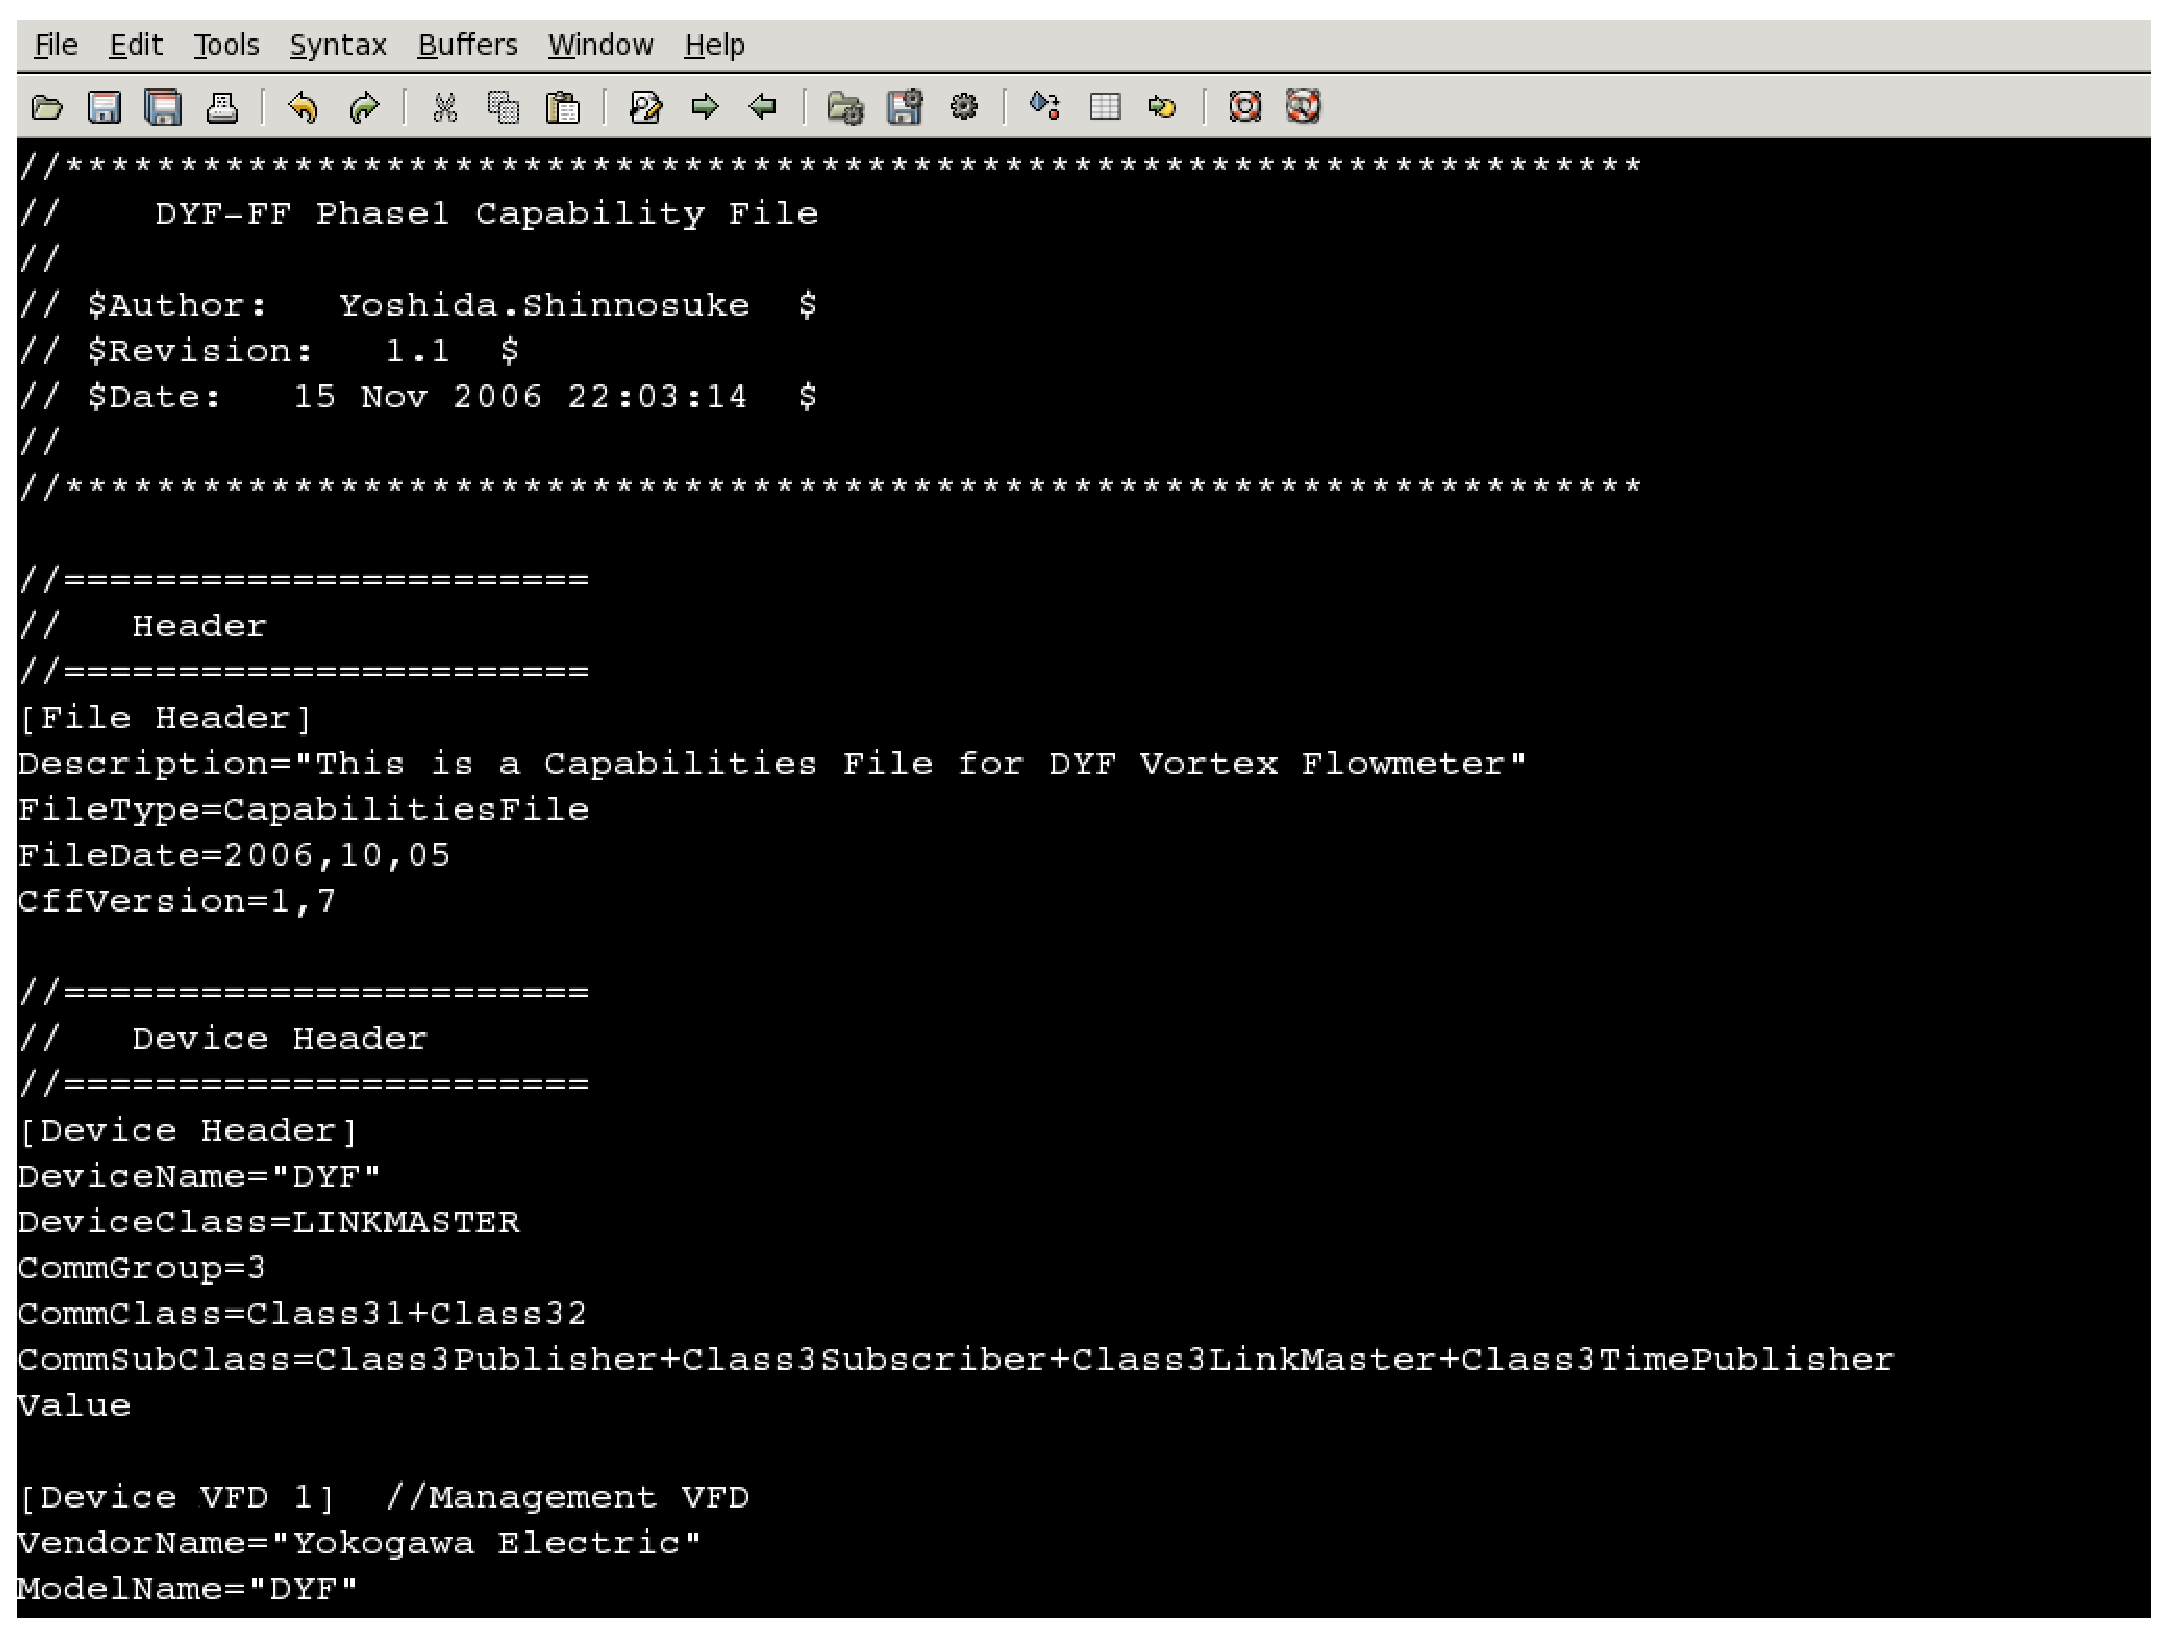
\includegraphics[width=6in]{fieldbus_30.eps}$$

\vskip 10pt

As with ``driver'' files needed to make a personal computer peripheral device function, it is important to have the correct versions of the Capability and DD files installed on the host system computer before attempting to commission the device.  It is permissible to have Capability and DD files installed that are newer than the physical device, but not vice-versa (a newer physical device than the Capability and DD files).  This requirement of proper configuration file management is a new task for the instrument technician and engineer to manage in their jobs.  With every new FF device installed in a control system, the proper configuration files must be obtained, installed, and archived for safe keeping in the event of data loss (a ``crash'') in the host system.








\filbreak
\subsection{Device commissioning}

This section illustrates the commissioning of a Fieldbus device on a real segment, showing screenshots of a host system's configuration menus.  The particular device happens to be a Fisher DVC5000f valve positioner, and the host system is a \textit{DeltaV} distributed control system manufactured by Emerson.  All configuration files were updated in this system prior to the commissioning exercise.  Keep in mind that the particular steps taken to commission any FF device will vary from one host system to another, and may not follow the sequence of steps shown here.  \index{Emerson DeltaV distributed control system (DCS)}

\filbreak

If an unconfigured FF device is connected to an H1 network, it appears as a ``decommissioned'' device.  On the Emerson DeltaV host system, all decommissioned FF devices appear within a designated folder on the ``container'' hierarchy.  Here, my Fisher DVC5000 device is shown highlighted in blue.  A commissioned FF device appears just below it (PT\_501), showing all available function blocks within that instrument:

$$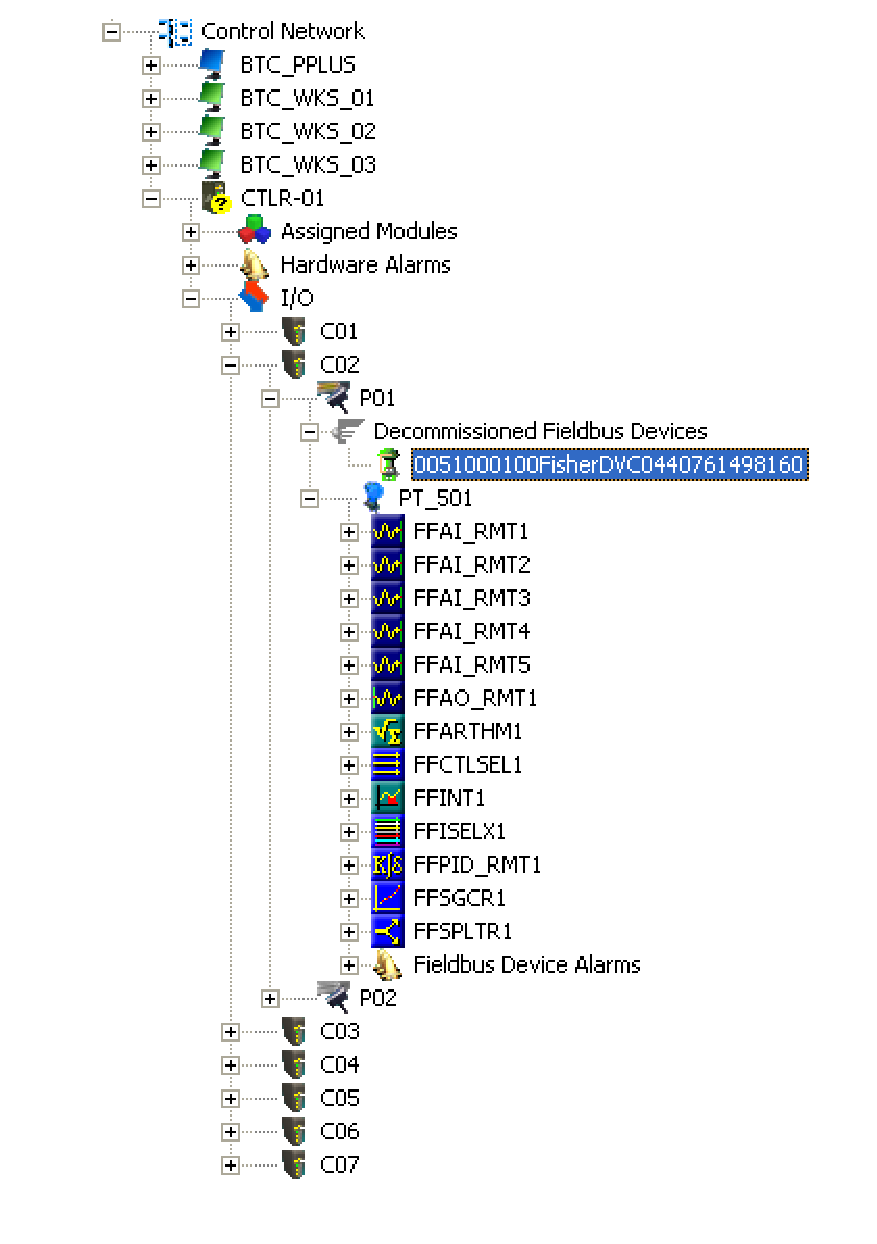
\includegraphics[height=6in]{fieldbus_14.eps}$$  % This graphic is 404 pixels wide and 580 pixels tall

\filbreak

Before any FF device may be recognized by the DeltaV host system, a ``placeholder'' and tag name must be created for it within the segment hierarchy.  To do this, a ``New Fieldbus Device'' must be added to the H1 port.  Once this option is selected\footnote{On the Emerson DeltaV system, most options are available as drop-down menu selections following a right-mouse-button click on the appropriate icon.}, a window opens up to allow naming of this new device:

$$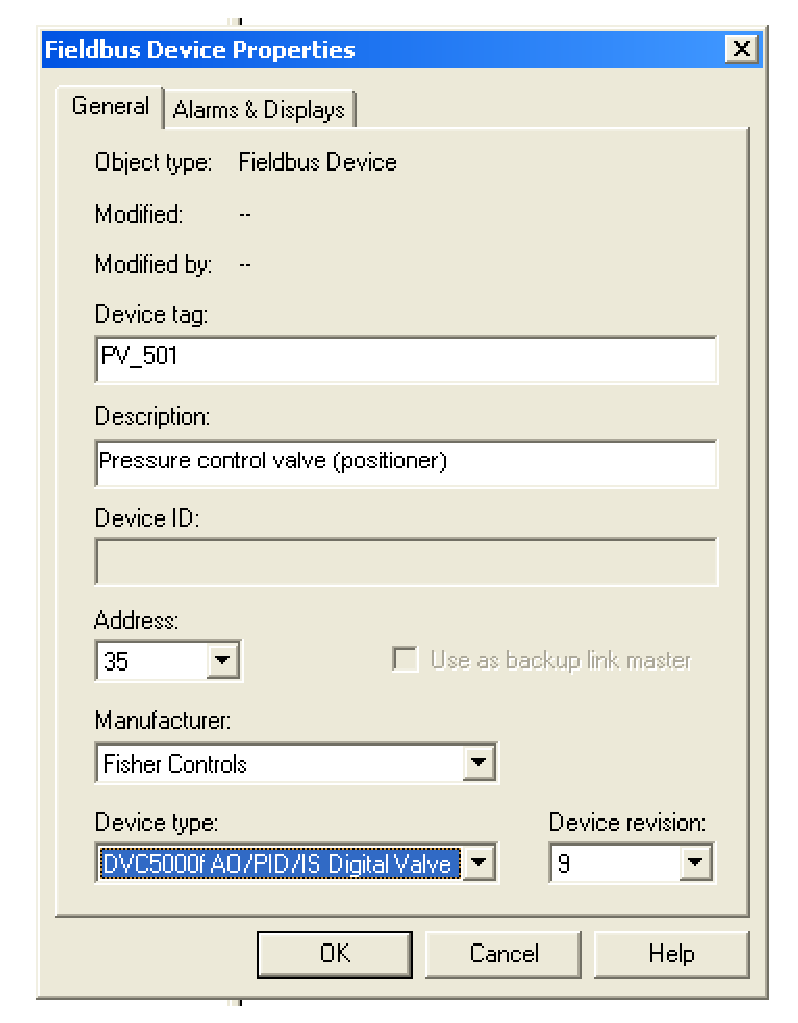
\includegraphics[height=5in]{fieldbus_13.eps}$$  % This graphic is 366 pixels wide and 474 pixels tall

Here, the tag name ``PV\_501'' has been chosen for the Fisher valve positioner, since it will work in conjunction with the pressure transmitter PT\_501 to form a complete pressure control loop.  In addition to a tag name (PV\_501), I have also added a text description (``Pressure control valve (positioner)''), and specified the device type (Fisher DVC5000f with AO, PID, and IS function block capability).  The DeltaV host system chose a free address for this device (35), although it is possible to manually select the desired device address at this point.  Note the ``Backup Link Master'' check box in this configuration window, which is grey in color (indicating the option is not available with this device).

\filbreak

After the device information has been entered for the new tag name, a ``placeholder'' icon appears within the hierarchy for the H1 segment (connected to Port 1).  You can see the new tag name (PV\_501) below the last function block for the commissioned FF instrument (PT\_501).  The actual device is still decommissioned, and appears as such:

$$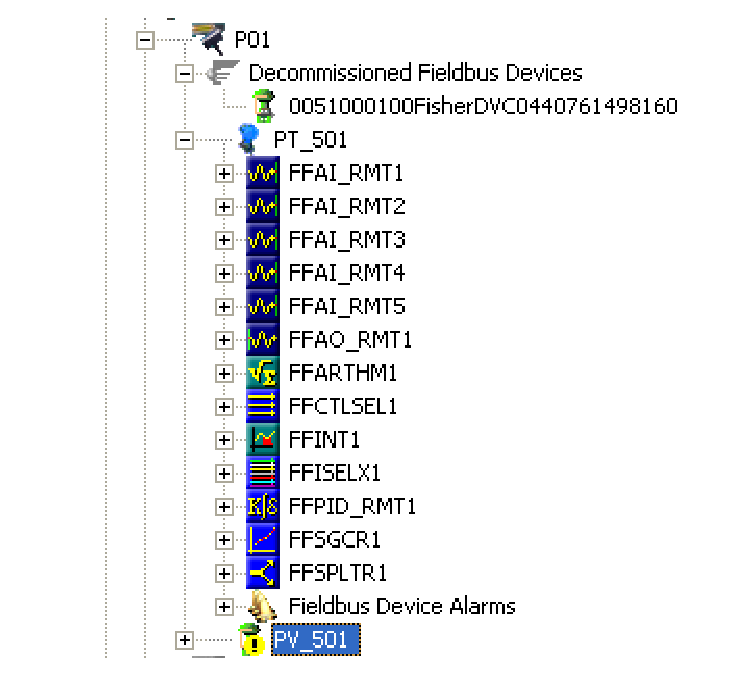
\includegraphics[height=3.18in]{fieldbus_15.eps}$$  % This graphic is 342 pixels wide and 307 pixels tall

\filbreak

By right-clicking on the new tag name and selecting the ``Commission'' option, a new window opens to allow you to select which decommissioned device should be given the new tag name.  Since there is only one decommissioned device on this particular H1 segment, only one option appears within the window:

$$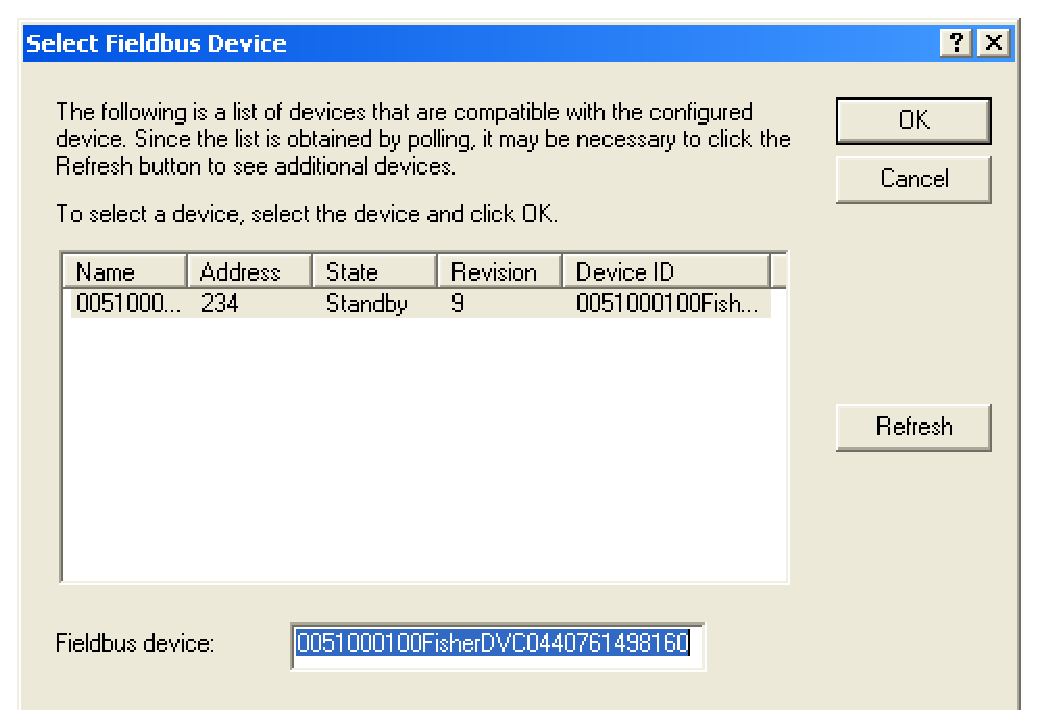
\includegraphics[width=6in]{fieldbus_16.eps}$$  % This graphic is 482 pixels wide and 332 pixels tall

\filbreak

After selecting the decommissioned device you wish to commission, the DeltaV host system prompts you to reconcile any differences between the newly created tag name placeholder and the decommissioned device.  If you want to use the existing values stored within the physical (decommissioned) device, you skip the ``reconcile'' step.  If you want to alter the values in the device from what they presently are, you choose the ``reconcile'' option which then opens up an editing window where you can set the device values however you wish.

$$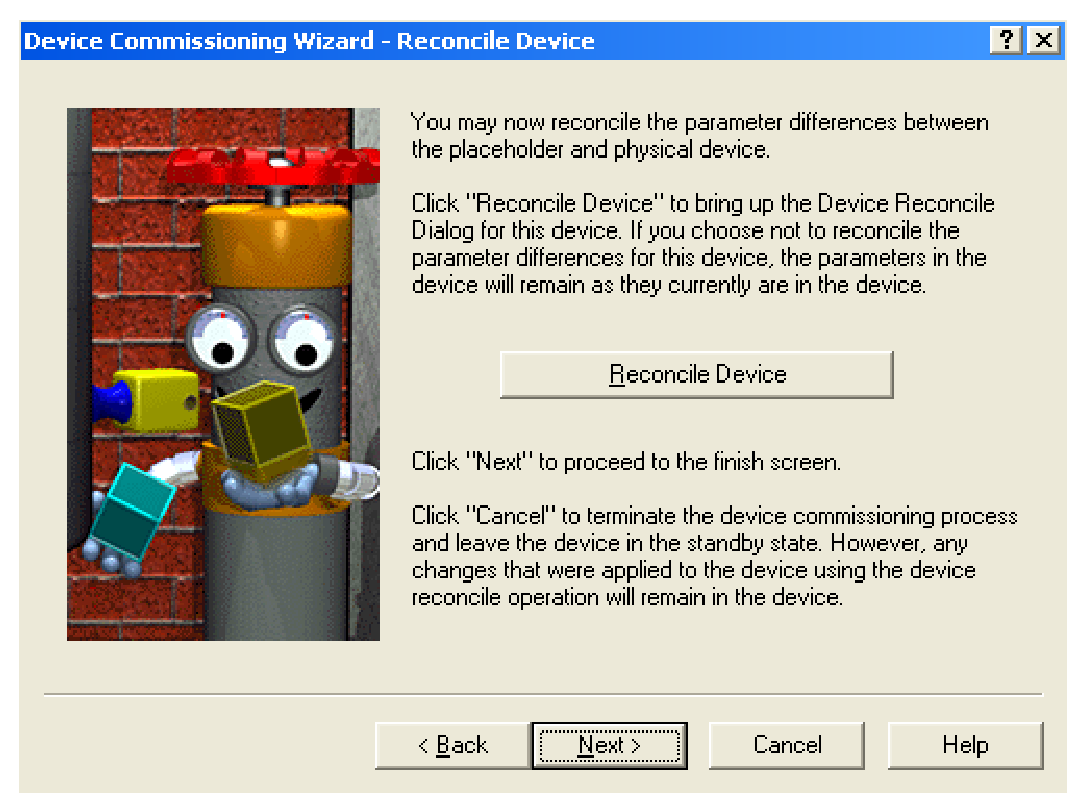
\includegraphics[width=6in]{fieldbus_17.eps}$$  % This graphic is 504 pixels wide and 372 pixels tall

\filbreak

After selecting (or not selecting) the ``reconcile'' option, the DeltaV system prompts you to confirm commissioning of the device, after which it goes through a series of animated\footnote{Animated graphics on the Emerson DeltaV control system prominently feature an anthropomorphized globe valve named Duncan.  There's nothing like a computer programmer with a sense of humor . . .} display sequences as the device transitions from the ``Standby'' state to the ``Commissioned'' state:

$$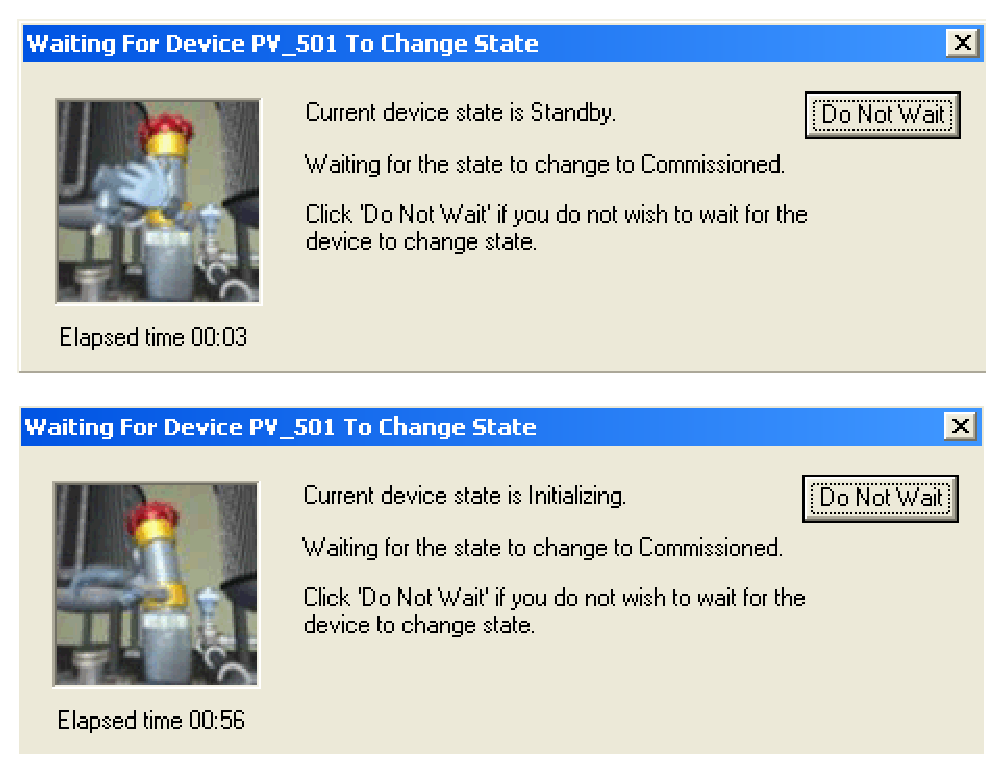
\includegraphics[width=5.5in]{fieldbus_18.eps}$$  % This graphic is 465 pixels wide and 353 pixels tall

As you can see, the commissioning process is not very fast.  After nearly one full minute of waiting, the device is still ``Initializing'' and not yet ``Commissioned.''  The network speed of 31.25 kbps and the priority of scheduled communications are limiting factors when exchanging large quantities of configuration data over a FF H1 network segment.  In order for device configuration to not interrupt or slow down process-critical data transfers, all configuration data exchanges must wait for unscheduled time periods, and then transmit at the relatively slow rate of 31.25 kbps when the alloted times arrive.  Any technician accustomed to the fast data transfer rates of modern Ethernet devices will feel as though he or she has taken a step back in time when computers were \textit{much} slower.  \index{Ethernet}

\filbreak

After commissioning this device on the DeltaV host system, several placeholders in the hierarchy appear with blue triangles next to them.  In the DeltaV system, these blue triangle icons represent the need to download database changes to the distributed nodes of the system:

$$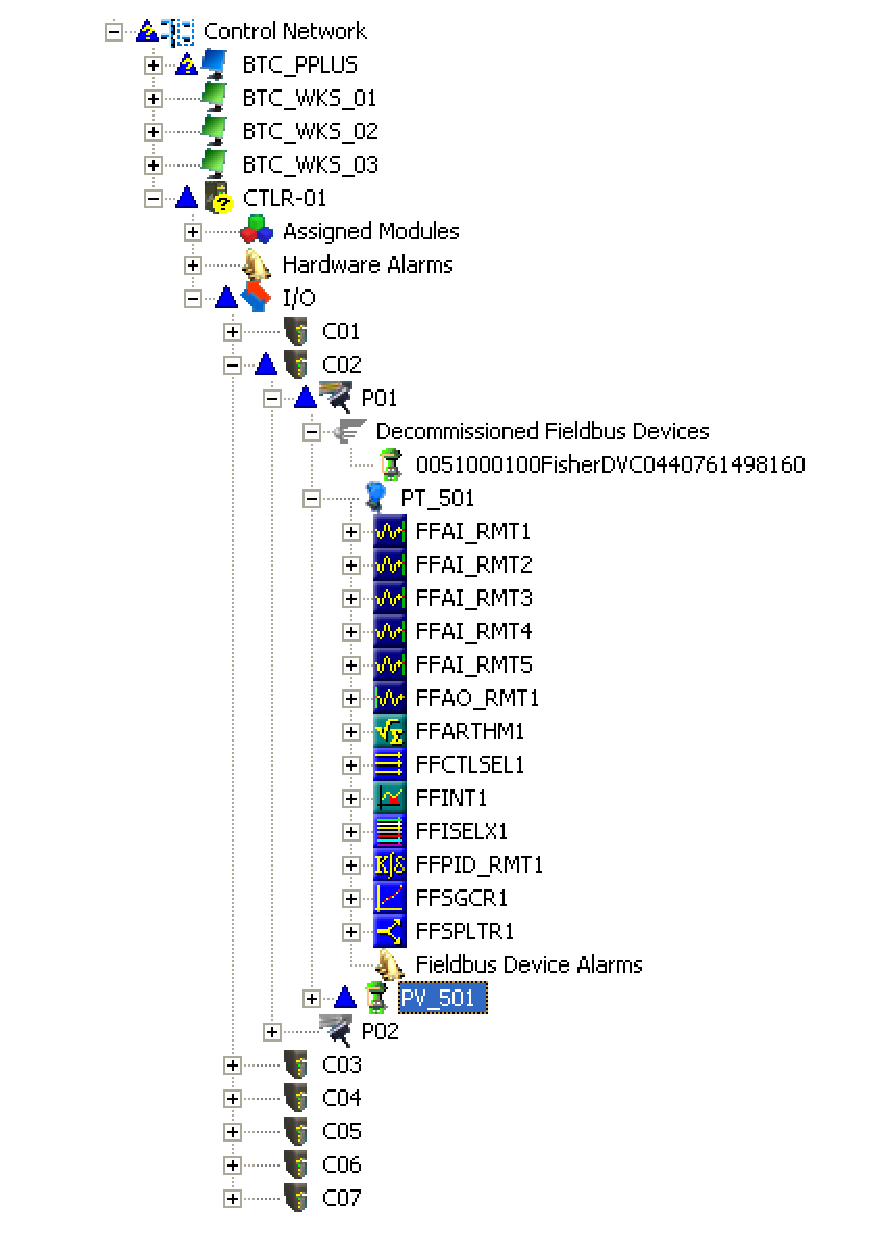
\includegraphics[height=6in]{fieldbus_19.eps}$$  % This graphic is 405 pixels wide and 580 pixels tall

\filbreak

After ``downloading'' the data, the new FF valve positioner shows up directly below the existing pressure transmitter as a commissioned instrument, and is ready for service.  The function blocks for pressure transmitter PT\_501 have been ``collapsed'' back into the transmitter's icon, and the function blocks for the new valve positioner (PV\_501) have been ``expanded'' for view:

$$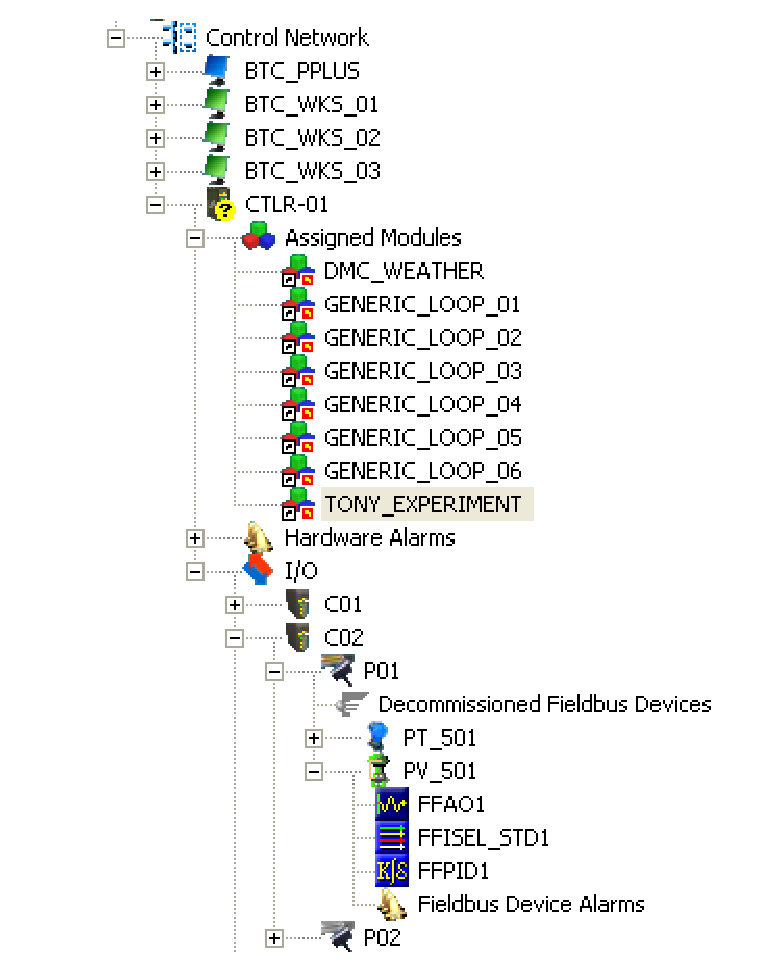
\includegraphics[height=4.63in]{fieldbus_20.eps}$$  % This graphic is 353 pixels wide and 448 pixels tall

As you can see, the new instrument (PV\_501) does not offer nearly as many function blocks as the original FF instrument (PT\_501).  The number of Fieldbus function blocks offered by any FF instrument is a function of that instrument's computational ability, internal task loading, and the discretion of its designers.  Obviously, this is an important factor to consider when designing a FF segment: being sure to include instruments that contain all the necessary function blocks to execute the desired control scheme.  This may also become an issue if one of the FF instruments in a control scheme is replaced with one of a different manufacturer or model, having fewer available function blocks.  If one or more mission-critical function blocks is not available in the replacement instrument, a different replacement must be sought.





\filbreak
\subsection{Calibration and ranging}

\label{FF transmitter calibration}

Calibration and ranging for a FF device is similar in principle to any other ``smart'' measurement instrument.  Unlike analog instruments, where the ``zero'' and ``span'' adjustments completely define the instrument's calibration \textit{and} range, calibration and ranging are two completely different functions in a digital instrument.

To begin, we will examine a block diagram of an analog pressure transmitter showing the zero and span adjustments, with analog signaling between all functions inside the transmitter:

$$\includegraphics{calibrate04.eps}$$

The ``zero'' and ``span'' adjustments together define the mathematical relationship between sensed pressure and current output.  Calibration of an analog transmitter consists of applying known (reference standard) input stimuli to the instrument, and adjusting the ``zero'' and ``span'' settings until the desired current output values are achieved.  The goal in doing this is to ensure accuracy of measurement.

The ``range'' of a transmitter is simply the input values associated with 0\% and 100\% output signals (e.g. 4 mA and 20 mA).  Ranging an analog transmitter consists (also) of adjusting the ``zero'' and ``span'' settings until the output signal corresponds to the desired LRV and URV points of the measured variable.  For an analog transmitter, the functions of ranging and calibration are always performed by the technician at the same time: to calibrate an analog transmitter is to range it, and vice-versa.

\filbreak

By contrast, a ``smart'' (digital) transmitter equipped with an analog 4-20 mA current output distinctly separates the calibration and range functions, each function determined by a different set of adjustments:

$$\includegraphics{calibrate03.eps}$$

Calibration of a ``smart'' transmitter consists of applying known (reference standard) input stimuli to the instrument and engaging the ``trim'' functions until the instrument accurately registers the input stimuli.  For a ``smart'' transmitter equipped with analog electronic (4-20 mA) output, there are \textit{two} sets of calibration trim adjustments: one for the analog-to-digital converter and another for the digital-to-analog converter.

Ranging, by contrast, establishes the mathematical relationship between the measured input value and the output current value.  To illustrate the difference between calibration and ranging, consider a case where a pressure transmitter is used to measure water pressure in a pipe.  Suppose the transmitter's pressure range of 0 to 100 PSI translates to a 4-20 mA output current.  If we desired to re-range an analog transmitter to measure a greater span of pressures (say, 0 to 150 PSI), we would have to re-apply known pressures of 0 PSI and 150 PSI while adjusting the zero and span potentiometers so 0 PSI input gave a 4 mA output value and 150 PSI input gave a 20 mA output value.  The only way to re-range an analog transmitter is to completely re-calibrate it.

In a ``smart'' (digital) measuring instrument, however, calibration against a known (standard) source need only be done at the specified intervals to ensure accuracy over long periods of time given the instrument's inevitable drift.  If our hypothetical transmitter were recently calibrated against a known pressure standard and trusted not to have drifted since the last calibration cycle, we could re-range it by simply changing the URV (upper range value) so that an applied pressure of 150 PSI now commands it to output 20 mA instead of an applied pressure of 100 PSI as was required before.  Digital instrumentation allows us to re-range without re-calibrating, representing a tremendous savings in technician time and effort.

\vskip 10pt

The distinction between \textit{calibration} and \textit{ranging} tends to confuse people, even some experienced technicians.  When working with an analog transmitter, you cannot calibrate without setting the instrument's range as well: the two functions are merged in the same procedures of adjusting zero and span.  When working with a digital transmitter, however, the function of calibration and the function of ranging are entirely separate.

For a detailed analogy explaining the distinction between calibration and ranging, refer to section \ref{calibration_versus_ranging} beginning on page \pageref{calibration_versus_ranging}.

\filbreak

Fieldbus instruments, of course, are ``smart'' in the same way, and their internal block diagrams look much the same as the ``smart'' transmitters with analog current output, albeit with a far greater number of parameters within each block.  The rectangle labeled ``XD'' in the following diagram is the Transducer block, while the rectangle labeled ``AI'' is the Analog Input block:

$$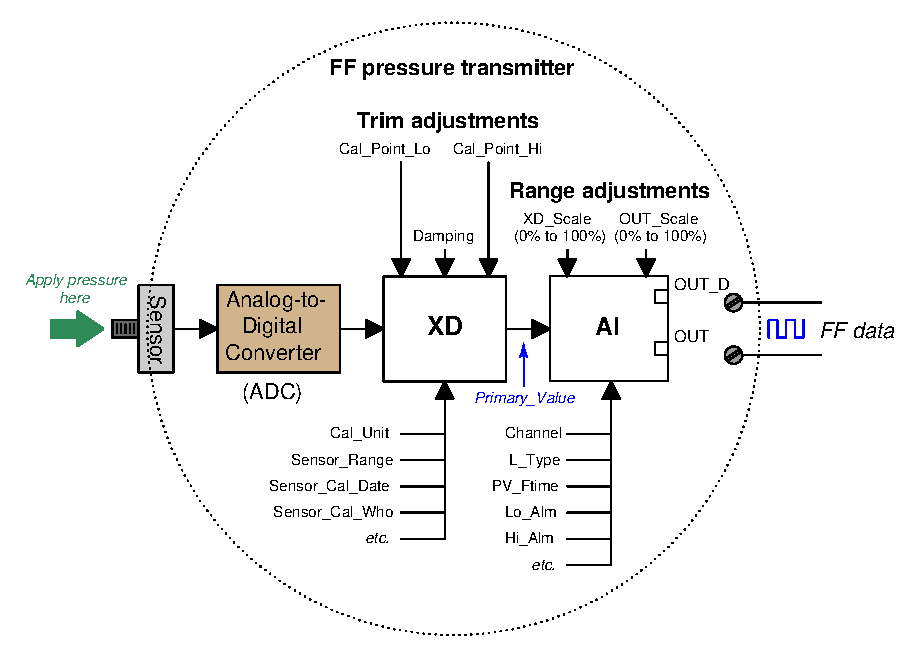
\includegraphics{fieldbus_31.eps}$$

Calibration (trim) values are set in the transducer block along with the engineering unit, making the output of the transducer block a digital value scaled in real units of measurement (e.g. PSI, kPa, bar, mm Hg, etc.) rather than an abstract ADC ``count'' value.  The analog input function block's \texttt{Channel} parameter tells it which transducer output to receive\footnote{Fieldbus transmitters often have multiple channels of measurement data to select from.  For example, the multi-variable Rosemount 3095MV transmitter assigns channel 1 as differential pressure, channel 2 as static pressure, channel 3 as process temperature, channel 4 as sensor temperature, and channel 5 as calculated mass flow.  Setting the \texttt{Channel} parameter properly in the AI block is therefore critical for linking it to the proper measurement variable.} as the pre-scaled ``Primary Value'', which it may then translate to another scaled value based on a proportionality between transducer scale values (\texttt{XD\_Scale} high and low) and output scale values (\texttt{OUT\_Scale} high and low).  

\vskip 10pt

To calibrate such a transmitter, the transducer block should first be placed in \textit{Out Of Service} (OOS) mode using a handheld FF communicator or the Fieldbus host system.  Next, a standard (calibration-grade) fluid pressure is applied to the transmitter's sensor and the \texttt{Cal\_Point\_Lo} parameter is set to equal this applied pressure.  After that, a greater pressure is applied to the sensor and the \texttt{Cal\_Point\_Hi} parameter is set to equal this applied pressure.  After setting the various calibration record-keeping parameters (e.g. \texttt{Sensor\_Cal\_Date}, \texttt{Sensor\_Cal\_Who}), the transducer block's mode may be returned to \textit{Auto} and the transmitter used once again.  \index{Out Of Service (OOS) mode, Fieldbus}  \index{OOS mode, Fieldbus}

To range such a transmitter, a correspondence between sensed pressure and the process variable must be determined and entered into the analog input function block's \texttt{XD\_Scale} and \texttt{OUT\_Scale} parameters.  If the pressure transmitter is being used to indirectly measure something other than pressure, these range parameters will become very useful, not only proportioning the numerical values of the measurement, but also casting the final digital output value into the desired ``engineering units'' (units of measurement).   \index{Engineering units}

\vskip 10pt

Ranging in Fieldbus transmitters is a somewhat confusing topic due to the unfortunate names given to the different \texttt{L\_Type} parameter options.  Here is a list of the \texttt{L\_Type} parameter options along with their meanings:

\begin{itemize}
\item \underbar{Direct} = the AI block will publish the signal output by the XD block, regardless of the specified \texttt{OUT\_Scale} range
\item \underbar{Indirect} = the AI block will mathematically scale the signal from the XD block into a range specified by \texttt{OUT\_Scale} parameters using a linear equation (e.g. $y = mx + b$)
\item \underbar{Indirect square root} = same as above, except that a square-root function is applied to the percentage of range (useful when characterizing flow transmitters based on differential pressure measurement)
\end{itemize}

\index{Channel, FOUNDATION Fieldbus AI block parameter}  \index{L\_Type, FOUNDATION Fieldbus AI block parameter}  \index{XD\_Scale, FOUNDATION Fieldbus AI block parameter}  \index{OUT\_Scale, FOUNDATION Fieldbus AI block parameter}

The terms ``direct'' and ``indirect'' are unfortunate\footnote{If I were king for a day, I would change the labels ``direct'' and ``indirect'' to ``raw'' and ``scaled'', respectively.  Alternatively, I would abandon the ``direct'' option altogether, because even when this option is chosen the \texttt{OUT\_Scale} range still exists and may contain ``scaled'' values even though these are ignored in ``direct'' mode!}, because they often cause people to interpret them as ``direct'' and ``reverse'' (as though \texttt{L\_Type} described the \textit{direction of action} for the function block).  This is \textit{not} what these terms mean for the AI block!  What a ``direct'' value for \texttt{L\_Type} means is that the \textit{raw} value of the XD block is what will be published onto the Fieldbus network by the AI block.  What an ``indirect'' value for \texttt{L\_Type} means is that the XD block's signal will be \textit{scaled} to a different range (specified by the \texttt{OUT\_Scale} parameter).  In summary, the technician must set the \texttt{XD\_Scale} range according to the primary signal sensed by the transmitter's sensing element, and set the \texttt{OUT\_Scale} range according to what the rest of the control system needs to see proportional to that primary signal.

\filbreak

The concept of ranging a FF transmitter makes more sense when viewed in the context of a real application.  Consider this example, where a pressure transmitter is being used to measure the level of ethanol (ethyl alcohol) stored in a 40 foot high tank.  The transmitter connects to the bottom of the tank by a tube, and is situated 10 feet below the tank bottom:

$$\includegraphics{fieldbus_32.eps}$$

\filbreak

Hydrostatic pressure exerted on the transmitter's sensing element is the product of liquid density ($\gamma$) and vertical liquid column height ($h$).  When the tank is empty, there will still be a vertical column of ethanol 10 feet high applying pressure to the transmitter's ``high'' pressure port.  Therefore, the pressure seen by the transmitter in an ``empty'' condition is equal to:

$$P_{empty} = \gamma h_{empty} = (49.3 \hbox{ lb/ft}^3) (10 \hbox{ ft})$$

$$P_{empty} = 493 \hbox{ lb/ft}^2 = 3.424 \hbox{ PSI}$$

\filbreak

When the tank is completely full (40 feet), the transmitter sees a vertical column of ethanol 50 feet high (the tank's 40 foot height plus the suppression height of 10 feet created by the transmitter's location below the tank bottom).  Therefore, the pressure seen by the transmitter in a ``full'' condition is equal to:

$$P_{full} = \gamma h_{full} = (49.3 \hbox{ lb/ft}^3) (40 \hbox{ ft} + 10 \hbox{ ft})$$

$$P_{full} = 2465 \hbox{ lb/ft}^2 = 17.12 \hbox{ PSI}$$

Thus, the transducer (XD) block in this Fieldbus transmitter will sense a liquid pressure ranging from 3.424 PSI to 17.12 PSI over the full range of the tank's storage capacity.

\filbreak

However, we do not want this transmitter to publish a signal to the Fieldbus network in units of PSI, because the operations personnel monitoring this control system want to see a measurement of ethanol \textit{level} inside the tank, not hydrostatic \textit{pressure} at the bottom of the tank.  We may be exploiting the principle of hydrostatic pressure to sense ethanol level, but we do not wish to report this measurement as a pressure.

The proper solution for this application is to set the \texttt{L\_Type} parameter to ``indirect'' which will instruct the AI function block to mathematically scale the XD block's pressure signal into a different range.  Then, we must specify\footnote{It is important to note that \textit{you} must correctly calculate the corresponding \texttt{XD\_Scale} and \texttt{OUT\_Scale} parameter values in order for this to work.  The Fieldbus instrument does not calculate the parameters for you, because it does not ``know'' how many PSI correspond to how many feet of liquid level in the tank.  These values must be calculated by some knowledgeable human technician or engineer and then entered into the instrument's AI block, after which the instrument will execute the specified scaling as a purely mathematical function.} the expected pressure range and its corresponding level range as \texttt{XD\_Scale} and \texttt{OUT\_Scale}, respectively\footnote{When configuring the \texttt{XD\_Scale} high and low range values, be sure to maintain consistency with the transducer block's \texttt{Primary\_Value\_Range} parameter unit.  Errors may result from mis-matched measurement units between the transducer block's measurement channel and the analog input block's \texttt{XD\_Scale} parameter.}:

% No blank lines allowed between lines of an \halign structure!
% I use comments (%) instead, so that TeX doesn't choke.

$$\vbox{\offinterlineskip
\halign{\strut
\vrule \quad\hfil # \ \hfil & 
\vrule \quad\hfil # \ \hfil \vrule \cr
\noalign{\hrule}
%
% First row
\textbf{AI block parameter} & \textbf{Range values} \cr
%
\noalign{\hrule}
%
% Another row
\texttt{L\_Type} & Indirect \cr
%
\noalign{\hrule}
%
% Another row
\texttt{XD\_Scale} & 3.424 PSI to 17.12 PSI \cr
%
\noalign{\hrule}
%
% Another row
\texttt{OUT\_Scale} & 0 feet to 40 feet \cr
%
\noalign{\hrule}
} % End of \halign 
}$$ % End of \vbox

Now, the ethanol tank's level will be accurately represented by the FF transmitter's output, both in numeric value and measurement unit.  An empty tank generating a pressure of 3.424 PSI causes the transmitter to output a ``0 feet'' digital signal value, while a full tank generating 17.12 PSI of pressure causes the transmitter to output a ``40 feet'' digital signal value.  Any ethanol levels between 0 and 40 feet will likewise be represented proportionally by the transmitter.

If at some later time the decision is made to re-locate the transmitter so it no longer has a 10 foot ``suppression'' with regard to the tank bottom, the \texttt{XD\_Scale} parameters may be adjusted to reflect the corresponding shift in pressure range, and the transmitter will still accurately represent ethanol level from 0 feet to 40 feet, without re-calibrating or re-configuring anything else in the transmitter.  

If we wished, we could even mathematically determine the liquid \textit{volume} stored inside this ethanol tank at different sensed pressures, and then scale the AI block's \texttt{OUT\_Scale} parameter to report a volume in units of gallons, liters, cubic feet, or any other appropriate volume unit.  Using the ``indirect'' mode with appropriate \texttt{XD\_Scale} and \texttt{OUT\_Scale} parameter values gives us great flexibility in how the transmitter senses and represents process data.

\vskip 10pt

In summary, we set the \texttt{XD\_Scale} parameter to the physical range of measurement directly sensed by the transducer, we set the \texttt{OUT\_Scale} parameter to the corresponding range of measurement we wish the transmitter to report to the rest of the control system, and we set \texttt{L\_Type} to ``indirect'' to enable this translation from one range to another.  We should only use the ``direct'' \texttt{L\_Type} setting if the raw transducer range is appropriate to output to the rest of the control system (e.g. if the transmitter directly senses fluid pressure and we wish this very same pressure value to be published onto the Fieldbus network by the transmitter, with no scaling). 

\filbreak

Here is another Fieldbus transmitter ranging application, this time a differential pressure transmitter sensing pressure dropped across an orifice plate in order to infer the rate of flow for fluid inside the pipe.  The transmitter senses small amounts of pressure difference (expressed in a unit of pressure called \textit{inches water column}), but what we want it to report to the Fieldbus network is an actual flow rate in gallons per minute.  

If we happen to know that this orifice plate produces a pressure drop of 125 inches water column (125 "WC) at a flow rate of 350 gallons per minute (350 GPM), we could set up the scaling parameters as shown:

$$\includegraphics{fieldbus_34.eps}$$

% No blank lines allowed between lines of an \halign structure!
% I use comments (%) instead, so that TeX doesn't choke.

$$\vbox{\offinterlineskip
\halign{\strut
\vrule \quad\hfil # \ \hfil & 
\vrule \quad\hfil # \ \hfil \vrule \cr
\noalign{\hrule}
%
% First row
\textbf{AI block parameter} & \textbf{Range values} \cr
%
\noalign{\hrule}
%
% Another row
\texttt{L\_Type} & Indirect Square Root \cr
%
\noalign{\hrule}
%
% Another row
\texttt{XD\_Scale} & 0 inches water to 125 inches water \cr
%
\noalign{\hrule}
%
% Another row
\texttt{OUT\_Scale} & 0 GPM to 350 GPM \cr
%
\noalign{\hrule}
} % End of \halign 
}$$ % End of \vbox

Note the use of the ``indirect \textit{square root}'' \texttt{L\_Type} parameter value instead of just ``indirect'' as we used in the ethanol tank example.  The square root function is necessary in this application because the relationship between differential pressure ($\Delta P$) and flow rate ($Q$) through an orifice is nonlinear, as described by the following formula:

$$Q = k \sqrt{\Delta P}$$

This particular nonlinearity is unique to pressure-based measurements of fluid flow, and does not find application in any other form of process measurement.

\vskip 10pt

As before, though, we see a common theme with the \texttt{XD\_Scale} and \texttt{OUT\_Scale} parameter ranges: we set the \texttt{XD\_Scale} parameter to the physical range of measurement directly sensed by the transducer, we set the \texttt{OUT\_Scale} parameter to the corresponding range of measurement we wish the transmitter to report to the rest of the control system, and we set \texttt{L\_Type} to ``indirect'' to enable this translation from one range to another.







\filbreak
\section{H1 FF segment troubleshooting}

Feedback obtained from industrial users of FF reveal a common pattern: Fieldbus is a powerful and reliable technology, but only if it is properly installed.  Poor installations, usually driven by a desire to minimize capital expenses, will cause numerous problems during commissioning and operation. 

One relatively easy way to avoid problems caused by short-circuits in FF wiring is to use coupling devices with built-in short-circuit protection.  This feature does not add significant cost to the coupling device, and it will prevent the entire segment from failing due to a short-circuit on a single spur cable or within a device.  Use coupling devices with indicator LEDs as well, since these give easy visual verification of network power which may greatly accelerate FF segment troubleshooting when the need arises.







\filbreak
\subsection{Cable resistance}

A simple check of an H1 segment's cabling consists of a series of resistance measurements performed with the segment unpowered (as is standard with any electrical resistance check), with all FF devices disconnected, and with the cable entirely disconnected (all three conductors) at the host end.  The following table shows guidelines published by the Fieldbus Foundation for H1 segment cable resistance measurements:

% No blank lines allowed between lines of an \halign structure!
% I use comments (%) instead, so that TeX doesn't choke.

$$\vbox{\offinterlineskip
\halign{\strut
\vrule \quad\hfil # \ \hfil & 
\vrule \quad\hfil # \ \hfil \vrule \cr
\noalign{\hrule}
%
% First row
\textbf{Measurement points} & \textbf{Expected resistance} \cr
%
\noalign{\hrule}
%
% Another row
Between (+) and ($-$) conductors & $>$ 50 k$\Omega$, increasing over time \cr
%
\noalign{\hrule}
%
% Another row
Between (+) conductor and shield (ground) & $>$ 20 M$\Omega$ \cr
%
\noalign{\hrule}
%
% Another row
Between ($-$) conductor and shield (ground) & $>$ 20 M$\Omega$ \cr
%
\noalign{\hrule}
%
% Another row
Between shield conductor and earth ground & $>$ 20 M$\Omega$ \cr
%
\noalign{\hrule}
} % End of \halign 
}$$ % End of \vbox

The last resistance check shown in the table checks for the presence of ground connections in the shield conductor \textit{other than} the one ground connection at the host end (which has been disconnected for the purposes of the test).  Since the shield should only be grounded at one point\footnote{An alternative method of shield grounding is to directly connect it to earth ground at one end, and then capacitively couple it to ground at other points along the segment length.  The capacitor(s) provide an AC path to ground for ``bleeding off'' any induced AC noise without providing a DC path which would cause a ground loop.} (to avoid ground loops), and this one point has been disconnected, the shield conductor should register no continuity with earth ground during the test.  \index{Ground loop}

The necessity of disconnecting all FF devices and host system interfaces is essential so that the resistance measurements reflect the health of the cable and nothing else.  The presence of any FF devices on the segment would substantially affect the resistance measurements, particularly resistance between the signal (+ and $-$) conductors.






\filbreak
\subsection{Signal strength}

The Fieldbus Foundation specifies a signal voltage (peak-to-peak) range of 350 mV to 700 mV for a healthy FF segment.  Excessive signal voltage levels point to a lack of terminator resistor(s), while insufficient voltage levels point to an over-abundance of terminators (or perhaps even a device short):

% No blank lines allowed between lines of an \halign structure!
% I use comments (%) instead, so that TeX doesn't choke.

$$\vbox{\offinterlineskip
\halign{\strut
\vrule \quad\hfil # \ \hfil & 
\vrule \quad\hfil # \ \hfil \vrule \cr
\noalign{\hrule}
%
% First row
\textbf{Signal voltage (pk-pk)} & \textbf{Interpretation} \cr
%
\noalign{\hrule}
%
% Another row
800 mV or more & Possibly missing terminator resistor \cr
%
\noalign{\hrule}
%
% Another row
350 mV to 700 mV & Good signal strength \cr
%
\noalign{\hrule}
%
% Another row
150 mV to 350 mV & Marginally low signal -- possible extra terminator resistor(s) \cr
%
\noalign{\hrule}
%
% Another row
150 mV or less & Too little signal to function \cr
%
\noalign{\hrule}
} % End of \halign 
}$$ % End of \vbox







\filbreak
\subsection{Electrical noise}

FF, like all digital networks, are unaffected by noise voltage below a certain threshold.  If noise voltage is present in excessive quantity, though, it may cause bits to be misinterpreted, causing data errors.  The Fieldbus Foundation gives the following recommendations\footnote{Bear in mind the tolerable level for noise will vary with signal voltage level as well.  All other factors being equal, a strong signal is less affected by the presence of noise than a weak signal (i.e. the signal-to-noise ratio, or \textit{SNR}, is crucial).} for noise voltage levels on a FF segment:

% No blank lines allowed between lines of an \halign structure!
% I use comments (%) instead, so that TeX doesn't choke.

$$\vbox{\offinterlineskip
\halign{\strut
\vrule \quad\hfil # \ \hfil & 
\vrule \quad\hfil # \ \hfil \vrule \cr
\noalign{\hrule}
%
% First row
\textbf{Noise voltage (pk-pk)} & \textbf{Interpretation} \cr
%
\noalign{\hrule}
%
% Another row
25 mV or less & Excellent \cr
%
\noalign{\hrule}
%
% Another row
25 mV to 50 mV & Okay \cr
%
\noalign{\hrule}
%
% Another row
50 mV to 100 mV & Marginal \cr
%
\noalign{\hrule}
%
% Another row
100 mV or more & Poor \cr
%
\noalign{\hrule}
} % End of \halign 
}$$ % End of \vbox

Fieldbus diagnostic tools measure noise on the network segment during times between message frames, when there should be purely DC voltage between the two conductors.







\filbreak
\subsection{Using an oscilloscope on H1 segments}

A tool available in most instrument shops is a digital-storage oscilloscope, which may be used to measure and display FF H1 signal waveforms for analysis of problems.  Analog oscilloscopes are also useful for network troubleshooting, but to a lesser degree\footnote{It is impossible to ``lock in'' (trigger) non-periodic waveforms on an analog oscilloscope, and so most network communications will appear as an incomprehensible blur when viewed on this kind of test instrument.  Digital oscilloscopes have the ability to ``capture'' and display momentary pulse streams, making it possible to ``freeze'' any portion of a network signal for visual analysis.}.

When using an oscilloscope to measure FF H1 signals, it is very important not to connect either of the FF segment conductors to earth ground through the oscilloscope.  Introducing such a ``ground fault'' to the network segment will almost certainly \textit{cause} communication problems, in addition to whatever problems already exist that compel you to diagnose with an oscilloscope.  If a single channel of the oscilloscope is connected across the segment wires, the ``ground'' clip of the probe will force one of those conductors to earth ground potential via the metal chassis of the oscilloscope which is grounded through the third prong of the power plug for safety.  An exception to this rule is if the oscilloscope itself is battery-powered and has an insulated case where no ground connection is made through the surface it sits on or the human hand that holds it.  Otherwise, using a single channel on a line-powered oscilloscope to measure network signals is inviting trouble.

\filbreak

If a line-powered oscilloscope must be used, the proper way to configure it is for \textit{differential channel} measurement.  In this mode, the oscilloscope will register the voltage \textit{between} two probe tips, rather than register the voltage between a single probe tip and earth ground.

$$\includegraphics{fieldbus_33.eps}$$

Configuring a dual-trace oscilloscope for differential mode is quite simple.  On the front panel of the oscilloscope, you must set the multi-trace controls to the \textit{Add} mode, where one trace on the screen represents the instantaneous sum of the two inputs (channels ``A'' and ``B'').  The volts per division ``sensitivity'' of both channels should be set to exactly the same value.  Also, the \textit{Invert} control must be engaged for the second input channel, forcing that channel's signal to be inverted (register upside-down on the screen).  The summation of channel ``A'' and an inverted channel ``B'' is equivalent to the mathematical difference (subtraction) between ``A'' and ``B,'' which means the single trace on the screen now represents the difference of potential between the two probe tips.  The oscilloscope now behaves as an ungrounded voltmeter, where neither of the test leads is referenced to earth ground.  \index{Oscilloscope, differential measurement mode}  \index{Differential measurement mode on an oscilloscope}








\filbreak
\subsection{Message re-transmissions}

Aside from voltage parameters (signal strength, noise amplitude), another good indicator of FF segment health is the number of message \textit{re-transmissions} over time.  Certain types of communication on an H1 segment require verification of a received signal (particularly client/server VCRs such as those used to communicate operator setpoint changes and diagnostic messages).  If the signal received by the client FF device appears corrupted, the device will request a \textit{re-transmission} of the message from the server device.  Re-transmission events, therefore, are an indication of how often messages are getting corrupted, which is a direct function of signal integrity in a Fieldbus segment.

Most host systems provide re-transmission statistics in much the same way that computers communicating via TCP/IP protocol have the ability to display the number of ``lost'' data packets over time.  Since nearly all FF segments function with a host system connected, this becomes a built-in diagnostic tool for technicians to troubleshoot FF network segments.

Hand-held diagnostic tools are also manufactured to detect signal voltage levels, noise voltage levels, and message re-transmissions.  Relcom manufactures both the model FBT-3 and model FBT-6 hand-held Fieldbus testers at the time of this writing (2009), the FBT-6 being the more capable of the two test devices.

% ADD: Relcom FBT-3 and FBT-6 Fieldbus monitors (FF only)
% ADD: Relcom FBT-5 Fieldbus Wiring Validator (FF or Profibus PA -- physical cable test only)








%\filbreak
%\section{Practical FF examples}

% ADD: examples of practical FF instrumentation systems
% ADD: show macrocycles with multiple loops (perhaps with repeated loops in one macrocycle?)
% ADD: Triple-redundant transmitters feeding into a signal selector!
% ADD: Cascaded level/flow or temperature/flow control system!
% ADD: Ratio (flow) control
% ADD: Boiler control (three-element): feedforward with trim
% ADD: Feedforward with dynamic compensation








\filbreak
\section{Review of fundamental principles}

Shown here is a partial listing of principles applied in the subject matter of this chapter, given for the purpose of expanding the reader's view of this chapter's concepts and of their general inter-relationships with concepts elsewhere in the book.  Your abilities as a problem-solver and as a life-long learner will be greatly enhanced by mastering the applications of these principles to a wide variety of topics, the more varied the better.

\begin{itemize}
\item \textbf{Analog vs. digital signals}: analog signals have infinite resolution but are susceptible to corruption by noise.  Digital signals have limited resolution but are tolerant of any noise measuring less than the difference in thresholds between the high and low states.
\item \textbf{Superposition theorem}: any linear, bilateral electrical network with multiple sources may be analyzed by taking one source at a time (while replacing all other sources with their internal impedance values) and analyzing all voltages and currents, then superimposing (summing) those voltage and current values to obtain the voltages and currents with all sources active.  Relevant to analyzing FOUNDATION Fieldbus H1 networks carrying DC power plus AC signals simultaneously.
\item \textbf{Transmission lines}: short-duration (pulsed) electrical signals travel along a cable at nearly the speed of light, reflecting off the end of that cable if not properly terminated.  Relevant to signal cables carrying high-frequency signals.
\end{itemize}











\filbreak
\section*{References}

% In alphabetical order!
% \noindent
% Lastname, Firstname MiddleI., \textit{Book Title}, Publisher, City, State, Year.
% \vskip 10pt
% \noindent
% Lastname, Firstname MiddleI., \textit{Book Title}, Publisher, City, State, Year.
% etc . . .

\vskip 10pt

\noindent
ANSI/ISA-5.1-2009, Instrumentation Symbols and Identification, Research Triangle Park, NC, 2009.

\vskip 10pt

\noindent
``Fieldbus Book -- A Tutorial'' (TI 38K02A01-01E) 1st Edition , Yokogawa Electric Corporation, Tokyo, Japan, 2001. 

\vskip 10pt

\noindent
``FOUNDATION Fieldbus Application Guide -- 31.25 kbit/s Intrinsically Safe Systems'' (AG 163) Revision 2.0, The Fieldbus Foundation, Austin, TX, 2004. 

\vskip 10pt

\noindent
``FOUNDATION Fieldbus Blocks'' (00809-0100-4783) Revision BA, Rosemount, Inc., Chanhassen, MN, 2000. 

\vskip 10pt

\noindent
``FOUNDATION Fieldbus System Engineering Guidelines'' (AG 181) Revision 2.0, The Fieldbus Foundation, Austin, TX, 2004. 

\vskip 10pt

\noindent
``FOUNDATION Specification System Architecture'' (FF 581) Revision FS 1.1, The Fieldbus Foundation, Austin, TX, 2000. 

\vskip 10pt

\noindent
Lipt\'ak, B\'ela G. et al., \textit{Instrument Engineers' Handbook -- Process Software and Digital Networks}, Third Edition, CRC Press, New York, NY, 2002.

\vskip 10pt

\noindent
``Model 3051 Transmitter with FOUNDATION Fieldbus'' (00809-0100-4774) Revision AA, Rosemount, Inc., Chanhassen, MN, 1999. 

\vskip 10pt

\noindent
``RSFieldbus -- Configuring and Programming Foundation Fieldbus Devices Application Guide'' (RSFBUS-AT001A-EN-E), Rockwell Software, Inc., Milwaukee, WI, 2004. 

\vskip 10pt

\noindent
Smith, John I., \textit{Modern Operational Circuit Design}, Wiley-Interscience, John Wiley \& Sons, Inc., New York, NY, 1971.

\vskip 10pt

\noindent
Park, John; Mackay, Steve; Wright, Edwin; \textit{Practical Data Communications for Instrumentation and Control}, IDC Technologies, published by Newnes (an imprint of Elsevier), Oxford, England, 2003.

\vskip 10pt

\noindent
``Rosemount 3095 MultiVariable Mass Flow Transmitter with HART or FOUNDATION Fieldbus Protocol'' (00809-0100-4716) Revision JA, Rosemount, Inc., Chanhassen, MN, 2008.

\vskip 10pt

\noindent
``The FOUNDATION Fieldbus Primer'' Revision 1.1, Fieldbus Inc., Austin, TX, 2001. 

\vskip 10pt

\noindent
``Wiring and Installation 31.25 kbit/s, Voltage Mode, Wire Medium Application Guide'' (AG-140) Revision 1.0, Fieldbus Foundation, Austin, TX, 2000. 














%%%%%%%%%%%%%%%%%%%%%%%%%%%%%%%%%%%%%%%%%%%%%%%%%%%%

